\documentclass[fontsize=12pt, paper=a4, headinclude, twoside=false, parskip=half+, pagesize=auto, numbers=noenddot, open=right, toc=listof, toc=bibliography]{scrreprt}
% PDF-Kompression
\pdfminorversion=5
\pdfobjcompresslevel=1
% Allgemeines
\usepackage[automark]{scrpage2} % Kopf- und Fußzeilen
\usepackage{amsmath,marvosym} % Mathesachen
\usepackage[T1]{fontenc} % Ligaturen, richtige Umlaute im PDF
\usepackage[utf8]{inputenc}% UTF8-Kodierung für Umlaute usw
% Schriften
\usepackage{mathpazo} % Palatino für Mathemodus
\usepackage{setspace} % Zeilenabstand
\onehalfspacing % 1,5 Zeilen
% Schriften-Größen
\setkomafont{chapter}{\Huge\rmfamily} % Überschrift der Ebene
\setkomafont{section}{\Large\rmfamily}
\setkomafont{subsection}{\large\rmfamily}
\setkomafont{subsubsection}{\large\rmfamily}
\setkomafont{chapterentry}{\large\rmfamily} % Überschrift der Ebene in Inhaltsverzeichnis
\setkomafont{descriptionlabel}{\bfseries\rmfamily} % für description Umgebungen
\setkomafont{captionlabel}{\small\bfseries}
\setkomafont{caption}{\small}
% Sprache: Deutsch
\usepackage[ngerman]{babel} % Silbentrennung
\usepackage{csquotes} % quotes
% PDF
\usepackage[ngerman]{hyperref}
\addto\extrasngerman{% Umbenennung der Kapitel Referenzen
  \def\subsectionautorefname{Abschnitt}%
  \def\subsubsectionautorefname{Abschnitt}%
}
\usepackage[final]{microtype} % mikrotypographische Optimierungen
\clubpenalty = 10000 
\widowpenalty = 10000 
\displaywidowpenalty = 10000
\usepackage{url}
\renewcommand*{\UrlFont}{\footnotesize}
\usepackage{pdflscape} % einzelne Seiten drehen können
% Tabellen
\usepackage{multirow} % Tabellen-Zellen über mehrere Zeilen
\usepackage{multicol} % mehre Spalten auf eine Seite
\usepackage{tabularx} % Für Tabellen mit vorgegeben Größen
\usepackage{longtable} % Tabellen über mehrere Seiten
\usepackage{array}
\usepackage{float}
%  Bibliographie
\usepackage{bibgerm} % Umlaute in BibTeX
\usepackage{natbib}
% Bilder
\usepackage{graphicx} % Bilder
\usepackage{color} % Farben
\usepackage{xcolor,colortbl} % Text Hintergrundfarben und Tabellenfarben
\usepackage{varwidth}
\usepackage{changepage}
\graphicspath{{images/}}
\DeclareGraphicsExtensions{.pdf,.png,.jpg} % bevorzuge pdf-Dateien
\usepackage{subcaption}  % mehrere Abbildungen nebeneinander/übereinander
\usepackage[all]{hypcap} % Beim Klicken auf Links zum Bild und nicht zu Caption gehen
% Bildunterschrift
\setcapindent{0em} % kein Einrücken der Caption von Figures und Tabellen
\setcapwidth{0.9\textwidth} % Breite der Caption nur 90% der Textbreite, damit sie sich vom restlichen Text abhebt
\setlength{\abovecaptionskip}{0.2cm} % Abstand der zwischen Bild- und Bildunterschrift
% Quellcode
\usepackage{listings} % für Formatierung in Quelltexten
\usepackage{DejaVuSansMono} % ttfamily font
\usepackage{todonotes}% Todo Notes
\presetkeys{todonotes}{inline}{}
% Bibliography multicoloumn
\usepackage{etoolbox}
\usepackage{relsize}
\patchcmd{\thebibliography}{\list}{\begin{multicols}{2}\small\list}{}{}\appto{\endthebibliography}{\end{multicols}}

\definecolor{gray}{rgb}{0.5,0.5,0.5}
\definecolor{orange}{rgb}{.99,0.5,0}
\definecolor{green}{rgb}{0,0.4,0}
\definecolor{lightgreen}{rgb}{0.7,1,0.7}
\definecolor{codegreen}{rgb}{0,0.6,0}
\definecolor{codegray}{rgb}{0.5,0.5,0.5}
\definecolor{backcolour}{rgb}{0.97,0.97,0.95}

\lstdefinestyle{mystyle}{
  inputencoding={utf8},
  xleftmargin=1em,
  backgroundcolor=\color{backcolour},   
  basicstyle=\tiny\ttfamily,
  commentstyle=\color{gray},
  keywordstyle=\color{green}\textbf,
  numberstyle=\tiny\color{codegray},
  stringstyle=\color{orange},
  breakautoindent  = true,
  breakindent      = 2em,
  breaklines       = true,
  postbreak        = ,
  prebreak         = \raisebox{-.8ex}[0ex][0ex]{\Righttorque},                
  captionpos=b,                    
  keepspaces=true,                 
  numbers=left,                    
  numbersep=5pt,
  numberstyle=\tiny\ttfamily\color{gray},               
  showspaces=false,                
  showstringspaces=false,
  showtabs=false,                  
  tabsize=2,
  literate=%
    {Ö}{{\"O}}1
    {Ä}{{\"A}}1
    {Ü}{{\"U}}1
    {ß}{{\ss}}1
    {ü}{{\"u}}1
    {ä}{{\"a}}1
    {ö}{{\"o}}1
    {~}{{\textasciitilde}}1
}
\lstset{style=mystyle}
% linksbündige Fußboten
\deffootnote{1.5em}{1em}{\makebox[1.5em][l]{\thefootnotemark}}

\typearea{14} % typearea berechnet einen sinnvollen Satzspiegel (das heißt die Seitenränder) siehe auch http://www.ctan.org/pkg/typearea. Diese Berechnung befindet sich am Schluss, damit die Einstellungen oben berücksichtigt werden
\textwidth=440pt % text width

\usepackage{scrhack} % Vermeidung einer Warnung
\usepackage{acronym} % Abkürzungsverzeichnis

% chapter margin
\renewcommand*{\chapterheadstartvskip}{\vspace*{0cm}}
\renewcommand*{\chapterheadendvskip}{\vspace{.5cm}}


% Eigene Befehle %%%%%%%%%%%%%%%%%%%%%%%%%%%%%%%%%%%%%%%%%%%%%%%%%5
% Matrix
\renewcommand*{\i}[1]{%
      {\textit{#1}}%
}
\renewcommand*{\b}[1]{%
      {\textbf{#1}}%
}
\renewcommand*{\tt}[1]{%
      {\footnotesize\texttt{#1}}%
}
\newcommand{\q}[1]{%
      {\enquote{#1}}%
}
\newcommand{\sq}[1]{%
      {\enquote*{#1}}%
}

% break inside a table cell
\newcommand{\br}[3]{%
      {\parbox{#1cm}{#2\\#3\vspace{3pt}}}%
}

\newcommand{\mat}[1]{%
      {\textbf{#1}}%
}
\newcommand{\info}[1]{
      {\colorbox{blue}{ (INFO: #1)}}
}
% Hinweis auf Programme in Datei
\newcommand{\datei}[1]{%
      {\ttfamily{#1}}%
}
\newcommand{\code}[1]{%
      {\footnotesize\ttfamily{\colorbox{gray!20}{\begin{varwidth}{\dimexpr\linewidth-2\fboxsep}#1\end{varwidth}}}}%
}
% bild mit defnierter Breite einfügen
\newcommand{\bild}[4]{
  \begin{figure}[H]
    \centering
      \vspace{1ex}
      \includegraphics[width=#2]{images/#1}
      \caption[#4]{\label{img.#1} #3}
    \vspace{1ex}
  \end{figure}
}
% bild mit defnierter Breite und Leftshift einfügen
\newcommand{\bildl}[5]{
  \begin{figure}[H]
    \centering
      \vspace{1ex}
      \hspace*{#3}
      \includegraphics[width=#2]{images/#1}
      \caption[#5]{\label{img.#1} #4}
    \vspace{1ex}
  \end{figure}
}
% bild mit eigener Breite
\newcommand{\bilda}[3]{
  \begin{figure}[H]
    \centering
      \vspace{1ex}
      \includegraphics{images/#1}
      \caption[#3]{\label{img.#1} #2}
      \vspace{1ex}
  \end{figure}
}
 % import preamble config
% start document
\begin{document}
\pagenumbering{Roman} % große Römische Seitenummerierung
\pagestyle{empty}

% title page
\clearscrheadings\clearscrplain
\begin{center}

\includegraphics[width=0.28\textwidth]{images/logo_tu_berlin}
\vspace{8mm}

{\huge Technische Universität Berlin}\\
\vspace{2mm}
{\large Quality and Usability Lab}\\
% \vspace{1mm}
% {\large Institute of Software Engineering\\and Theoretical Computer Science}\\
\vspace{11mm}

{\Huge Part-of-Speech Tagging\\[-2mm] with Neural Networks\\[-2mm] for a Conversational Agent\\}
\vspace{20mm}
{\Huge \b{Master Thesis}}\\
{\b{Master of Science (M.Sc.)}}\\
\vspace{24mm}
\begin{tabular}{rl}
  \b{Author} & Andreas Müller\\
  \b{Major} & Computer Engineering\\
  \b{Matriculation No.} & 333471\\
   & \\
  \b{Date} & ??? \\
  \b{1st supervisor} & Prof. Dr.-Ing. Sebastian Möller \\
  \b{2nd supervisor} & Prof. Dr. ??? \\
\end{tabular}

\end{center}
\clearpage
\pagestyle{useheadings} % normale Kopf- und Fußzeilen für den Rest

% ==================================================================================================
\BlankPage

% ==================================================================================================
\chapter*{Eidesstattliche Erklärung}
Hiermit versichere ich, dass ich die vorliegende Arbeit selbstständig verfasst und keine anderen als die angegebenen Quellen und Hilfsmittel benutzt habe. Alle Ausführungen, die anderen veröffentlichten oder nicht veröffentlichten Schriften wörtlich oder sinngemäß entnommen wurden, habe ich kenntlich gemacht.

Die Arbeit hat in gleicher oder ähnlicher Fassung noch keiner anderen Prüfungsbehörde vorgelegen.
\vspace{10mm}

Berlin, den \today\\

\vspace{1cm}
\rule{.5\textwidth}{.5pt}\\
Unterschrift

% ==================================================================================================
\BlankPage

% ==================================================================================================
\chapter*{Abstract}
...

% ==================================================================================================
\BlankPage

% ==================================================================================================
\chapter*{Zusammenfassung}
...

% ==================================================================================================
\BlankPage

% ==================================================================================================
\tableofcontents
% ==================================================================================================
\listoffigures
% ==================================================================================================
\listoftables

% ==================================================================================================
\chapter*{Abbreviations}\label{s.abbr}
\addcontentsline{toc}{chapter}{Abbreviations}
\markboth{Abbreviations}{Abbreviations}
\begin{acronym}[----------------]
 \acro{NLP}{\i{Natural Language Processing} (linguistische Datenverarbeitung)}
 \acro{IR}{\i{Information Retrieval} (Informationsrückgewinnung)}
 \acro{SGD}{\i{Stochastic Gradient Descent}}
 \acro{NNLM}{\i{(Feedforward) Neural Net Language Model}}
 \acro{RNNLM}{\i{Recurrent Neural Net Language Model}}
 \acro{CBOW}{\i{Continous Bag-of-Words}}
\end{acronym}


% Inhalt Beginn
% ==================================================================================================
\chapter{Introduction}\label{c.introduction}
\pagenumbering{arabic} % ab jetzt die normale arabische Nummerierung der Seiten
% Die Analyse und Verarbeitung von Texten natürlicher Sprache stellt die Grundlage für zahlreiche Anwendungen der linguistischen Datenverarbeitung (engl. \i{Natural Language Processing}, NLP) dar und ist heute ein zentrales Forschungsgebiet von Internetfirmen wie Facebook\footnote{Facebook veröffentlichte 2013 einen wissenschaftlichen Artikel zu \i{Unicorn} (Curtiss et al. \citep{Curtiss2013}), eines Indexing-System für Facebook's Graph Search, welche es ermöglicht, Suchanfragen der Art \i{"`Restaurants in San Francisco liked by people from Beijing"'} zu stellen.}, Google\footnote{Google kündigte Ende September 2013 \i{Hummingbird} an (Shapiro et al. \citep{Shapiro2013}), einen Algorithmus zur effizienteren Verarbeitung und Sortierung des Suchindex. Damit soll die Bedeutung eines Satzes besser verstanden werden, um präzisere Suchergebnisse komplexer Suchanfragen zu erreichen.} oder Yahoo\footnote{Yahoo kaufte Ende 2013 \i{SkyPhrase} (Miners et al. \citep{Miners2013}), ein NLP Start-Up, um die Verarbeitung und Resultate von Benutzeranfragen in vielen Yahoo-Anwendungen zu verbessern.}, denen große Mengen an Textdaten zur Verfügung stehen.

% NLP möchte im Allgemeinen die natürliche Sprache algorithmisch verarbeiten, sodass automatisiert unstrukturierte Daten in geordnete Informationen umgewandelt und gewünschte Informationen extrahiert werden können. Dieser Vorgang wird als \i{Information Retrieval} (IR) bezeichnet. Teil des IR ist die Information Extraction, welche gezielt Informationen einer bestimmten Vorgabe gewinnen möchte. Um natürliche Sprache automatisiert zu verarbeiten, müssen Wörter in ein geeignetes maschinenlesbares Format umgewandelt werden. Wort-Vektoren stellen eine Möglichkeit dar, Wörter numerisch zu beschreiben und ihren sprachlichen Zusammenhang durch die Beziehung der Vektoren in einem beschränkten Vektorraum abzubilden (Bengio et al., 2003 \citep{Bengio2003}).

% Sprach-Modellierung kann mithilfe verschiedener Ansätze realisiert werden. Zum einen gibt es einfache Modelle wie \i{Bag-of-Words} (BOW, vgl. \autoref{ss.bagofwords}) oder N-Gramme (vgl. \autoref{ss.ngram}). Die Größe des Vokabulars ist hier maßgebend für die Dimension der resultierenden Wort-Vektoren, sodass webbasierte Korpora (wie beispielsweise die freie Enzyklopädie Wikipedia) aufgrund ihrer Größe auch bei hoher Rechenleistung sehr lange Berechnungszeiten verursachen. Da z.B. beim BOW-Modell jedes neue Wort im Vokabular jedem Wort-Vektor eine weitere Dimension hinzufügt, verlieren folglich die Wort-Vektoren bezüglich des repräsentierten Wortes zunehmend an Bedeutung\footnote{Dieses Phänomen ist als \i{Curse of Dimensionality} – Fluch der Dimensionalität bekannt. Der Begriff wurde 1961 erstmals verwendet von R.E. Bellman \citep{Bellman1961}.}. Zum anderen gibt es beim \i{Deep Learning} den Ansatz der neuronalen Netzwerke, welche die Wort-Vektoren durch mehrschichtige Abstraktionen ohne Vorgabe trainieren können. Es wurde gezeigt, dass diese mithilfe von neuronalen Netzwerken gelernten Wort-Vektoren sprachliche Merkmale sehr gut abbilden konnten (Bengio et al., 2003 \citep{Bengio2003}). Dadurch war es möglich, komplexere Aufgaben zu lösen wie beispielsweise \i{Relation Detection}, \i{Relation Classification} (Zeng et al., 2014 \citep{Zeng2014}) oder \i{Sentiment Analysis} (Socher et al., 2013 \citep{Socher2013}).

% Viele Modelle wurden bisher fast ausschließlich für die englische Sprache trainiert, sodass es für die deutsche Sprache kaum Modelle gibt, mit deren Hilfe man Aussagen darüber treffen könnte, wie präzise deutsche Wort-Vektoren sind und welche Parameter genauere Ergebnisse auf einem deutschen Korpus erzielen. Aufgrund der sprachlichen Unterschiede zwischen Deutsch und Englisch können Ergebnisse englischer Sprachmodelle nicht ohne Weiteres für die deutsche Sprache übernommen werden. So gibt es im Deutschen beispielsweise männliche, weibliche und sächliche Artikel, wobei sich biologisches und grammatikalisches Geschlecht unterscheiden können. Gegenstände sind nicht wie im Englischen ausschließlich sächlich, sondern haben oft ein Geschlecht, wie \q{\b{der} Stuhl}  oder \q{\b{die} Lampe} (\i{\b{the} chair}, \i{\b{the} lamp}). Außerdem gibt es Unterschiede in der Wort-Reihenfolge: Während englische Sätze und Nebensätze immer dem Schema `Subjekt - Prädikat - Objekt' folgen, so steht in deutschen Nebensätzen das Verb an letzter Stelle, z.B. \q{Ich weiß, dass \b{sie} das Buch \b{liest}.} (\i{I know that \b{she} \b{reads} the book.}), wobei dem Verb auch längere Beschreibungen vorangestellt werden können. Werden Sprachmodelle aufgrund einer bestimmten Anzahl nebeneinander stehender Wörter (Fenster) trainiert, so ergeben sich für beide Sprachen schon wegen der Unterschiede in der Wort-Reihenfolge verschiedene Ergebnisse.

% Ziel dieser Arbeit ist es, die durch Variation verschiedener Parameter beim Modelltraining entstandenen deutschen Wort-Vektoren zu analysieren und zu evaluieren. Dazu wird ein Toolkit für Korpuserstellung, Training, Evaluation und Visualisierung entwickelt und für die Evaluation deutsche Test-Sets generiert. Dieses Toolkit, das finale Sprachmodell und die Test-Sets stehen anschließend als Grundlage für weiterführende Anwendungen deutscher Wort-Vektoren zur Verfügung.

% Anknüpfen soll diese Arbeit an die Ergebnisse des DIMA Projektes \q{Exploring semantic word similarities in German News Articles} \citep{Arras2014}, welches sich mit unüberwachtem Clustering deutscher Nachrichtenartikel beschäftigte. Basierend auf einem Korpus von 3 Millionen Nachrichtenartikeln wurden in diesem Projekt bereits verschiedene Modelle unter Parameter-Variation mithilfe eines neuronalen Netzwerks auf deutscher Sprache trainiert. Es wurde gezeigt, dass das Trainieren von Wort-Vektoren auf einem Korpus deutscher Sprache prinzipiell funktioniert, sodass darauf aufbauend in dieser Arbeit das beschriebene Toolkit zur Bewertung deutscher Modelle implementiert werden kann.

% Diese Arbeit ist in 6 Kapitel gegliedert. In \autoref{c.grundlagen} werden zunächst die Grundlagen zu Wort-Vektoren allgemein und maschinellem Lernen in der linguistischen Datenverarbeitung dargestellt. Anschließend wird in \autoref{c.neuronalenetzwerke} genauer auf den Aufbau neuronaler Netzwerke und darauf basierenden Architekturen und Modellen eingegangen. Das Training der Modelle und die daraus resultierenden verbesserten Wort-Vektoren werden hier erläutert. Die Umsetzung des praktischen Teils, der Implementierung eines Toolkits zur Korpora-Erstellung, Modelltraining und Evaluation trainierter Modelle, ist in \autoref{c.implementierung} dargestellt. Dabei werden durch Parametervariation verschiedene Modelle spezifiziert und die Erstellung von Test-Sets erläutert. In \autoref{c.auswertung} werden die Ergebnisse der trainierten Modelle sowie das daraus resultierende optimale Modell ausgewertet. Abschließend werden die wichtigsten Erkenntnisse in \autoref{c.fazit} zusammengefasst.

% Da es in dieser Arbeit um die Modellierung deutscher Sprache geht, werden weitestgehend die üblicherweise verwendeten deutschen Entsprechungen englischer Fachbegriffe verwendet.

% % ==================================================================================================
% \chapter{Grundlagen linguistischer Datenverarbeitung}\label{c.grundlagen}
% Dieses Kapitel gibt eine Einführung in die geschichtliche Entwicklung von Wort-Vektoren und neuronaler Netzwerke sowie grundlegende Konzepte der Verarbeitung und Modellierung natürlicher Sprache. Die linguistische Datenverarbeitung und neuronale Netzwerke bilden heute eine sehr großes Forschungsfeld, weshalb lediglich ein grober Überblick der Grundlagen dazu gegeben werden soll und der Fokus auf Wort-Vektoren als mögliche Repräsentation von geschriebener Sprache liegt.

% \section{Historischer Kontext von Wort-Vektoren}\label{s.historischerkontext}
% Das algorithmische Erlernen eines Wort-Vektors (oder allgemein der Darstellung eines Wortes) mittels neuronaler Netzwerke geht auf die Anfänge künstlicher neuronaler Netzwerke zurück. Frank Rosenblatt legte 1958 mit seinem Konvergenztheorem über das Perzeptron\footnote{Das Perzeptron ist ein von Frank Rosenblatt geprägter Begriff zur Bezeichnung eines einfachen künstlichen neuronalen Netzwerks mit zuerst nur einem einzelnen Neuron \citep{Rosenblatt1958}.} den Grundstein künstlicher, an das biologische Nervensystem angelehnter Netzwerke. Er zeigte, dass mit dem angegebenen Lernverfahren jede Funktion gelernt werden kann, die mit diesem Modell repräsentierbar ist \citep{Rosenblatt1958}. Anknüpfend wurde 1960 von Bernard Widrow das Adaline\footnote{Adaline ist ein Akronym für \i{Adaptive Linear Neuron}.}-Modell eines neuronalen Netzwerks vorgestellt, bei welchem bereits die Gewichte der Eingabe vom Lernalgorithmus angepasst werden konnten \citep{Widrow1960}. Mit einer Publikation von Marvin Minsky und Seymour Papert im Jahr 1969 wurden die Grenzen des einstufigen Perzeptrons gezeigt \citep{Minsky1969}. Es war demnach nicht möglich, eine XOR-Funktion zu repräsentieren, da diese nicht linear separierbar ist (XOR-Problem vgl. \autoref{img.xor}).

% \bild{xor}{11cm}{XOR-Problem: Es kann kein linearer Klassifikator $c_{linear}$ für das Ergebnis einer Entweder-Oder-Abfrage gefunden werden.}{XOR-Problem}

% In den folgenden Jahren nahm das Interesse der weiteren Erforschung künstlicher neuronaler Netzwerke ab. Mögliche Ursache dieser Entwicklung ist neben dem Aufzeigen der Mängel des Pezeptrons durch Minsky auch die Tatsache, dass die zu diesem Zeitpunkt verfügbare Rechenleistung der Computer nicht ausreichte, um repräsentative Modelle zu trainieren. Erst 1982 veröffentliche John Hopfield eine Publikation zu neuronalen Netzwerken mit Rückkopplung (Hopfield-Netze \citep{Hopfield1982}), wodurch Optimierungsprobleme wie das \i{Travelling Salesman Problem}\footnote{Das Problem des Handlungsreisenden oder Rundreiseproblem: Die Reihenfolge einmalig zu besuchender Orte soll so gewählt werden, dass der dabei zurückgelegte Weg minimal ist, wobei der letzte Ort wieder der Ausgangsort ist (Rundreise).} lösbar wurden. Eine Publikation von Rumelhart et al. zu Backpropagation 1986 \citep{Rumelhart1986} (vgl. \autoref{ss.backpropagation}) und die stetig steigende Rechenleistung\footnote{Die ersten Prozessoren basierend auf Transistortechnik (Mikroprozessoren) kamen 1971 auf den Markt und lösten die zuvor genutzte Röhrentechnik ab. Dies hatte zur Folge, dass Computer kleiner und preiswerter gebaut werden konnten, wobei die Rechenleistung deutlich zunahm.} führte zur Wiederbelebung der Erforschung künstlicher neuronaler Netzwerke. Trotzdem waren in den 1980er und 1990er Jahren noch zu wenig digitale Daten für ein erfolgreiches Training vorhanden.

% % 1990 wurde von Deerwester et al. \citep{Deerwester1990} die Latente Semantische Analyse (engl. \i{Latent Semantic Analysis} (LSA) oder \i{Latent Semantic Indexing} (LSI)) vorgestellt. Dabei handelt es sich um ein Verfahren, dass die durch Vektorraum-Retrieval\footnote{Zum Information-Retrieval gehörendes Verfahren, bei welchem die Merkmale (z.B. von Dokumenten) als Vektoren eines hochdimensionalen Raums dargestellt werden, wobei die Ähnlichkeit der Vektoren durch ihre Distanz repräsentiert wird. Ein gängiges Maß für diese Distanz ist hier die Kosinus-Ähnlichkeit.} gewonnene Term-Frequenz-Matrix mittels Singulärwertzerlegung approximiert und somit die Dimension der dort repräsentierten Terme (wie z.B. Dokumente) reduziert. Diese Dimensionsverringerung geschieht dabei durch Vereinen von Dimensionen ähnlicher Bedeutung, welche durch das Wiederauftreten von Termen in verschiedenen Dokumenten erkannt wird\footnote{Der entstehende geringere Vektorraum wird auch Semantischer Raum genannt}. Dadurch war es bereits möglich, automatisiert Dokumente anhand ihres Inhaltes zu klassifizieren.

% % Ein weitere Möglichkeit zur Modellierung von Dokumenten ist die 2003 von Blei et al. veröffentlichte \i{Latent Dirichlet Allocation} (LDA) \citep{Blei2012}. Als generatives Wahrscheinlichkeitsmodell kann LDA Dokumente klassifizieren, indem jedes Wort eines Dokuments einem oder mehreren vorgegebenen Themen zugeordnet wird. Die Zugehörigkeit eines Wortes zu einem Thema wird dabei iterativ über die Dirichlet-Verteilung gelernt.

% Mikolov et al. \citep{Mikolov2012} geben einen kurzen geschichtlichen Überblick über Modelle neuronaler Netzwerke. Demnach wurden 2003 (Bengio et al. \citep{Bengio2003}) und in den darauffolgenden Jahren durch neuronale Netzwerke trainierte Sprachmodelle vorgestellt, welche die klassische Aufgabe der Vorhersage einer Wahrscheinlichkeitsverteilung für ein Wort aufgrund seiner vorangehenden Wörter lösen sollten. Zunächst wurden diese mit Feedforward-Netzwerken erforscht \citep{Bengio2003}, später mit Recurrent-Netzwerken \citep{Mikolov2010} (vgl. \autoref{s.modelle}). Diese Sprachmodelle erzielten sehr gute Ergebnisse, allerdings war dafür auch für heutige Verhältnisse noch immer eine hohe Rechenleistung notwendig. Um mehr Trainingsdaten verarbeiten zu können, wurde folglich nach recheneffizienteren Modellen gesucht. Daraus entstanden Sprachmodelle, welche durch ein neuronales Netzwerk ohne verborgene Ebenen trainiert wurden, wie Continous Bag-of-Words und Skip-Gram (vgl. \autoref{s.modelle}).

% Nach mehr als 50 Jahren ist das Forschungsgebiet neuronaler Netzwerke heute sehr groß und hat eine Vielfalt von Anwendungsgebieten. So werden neuronale Netzwerke u.a. für Mustererkennung, Bildverarbeitung, Spracherkennung, Medizinische Diagnostik und Klangsynthese verwendet. Diese Arbeit behandelt dabei ausschließlich die Modellierung geschriebener Sprache.

% \section{Maschinelles Lernen für NLP}\label{s.maschinelleslernen}
% Im Allgemeinen bezeichnet maschinelles Lernen den Wissenserwerb eines künstlichen Systems, sodass das System anschließend verallgemeinern und das Wissen auf unbekannte Daten anwenden kann. Maschinelle Lernmethoden sind für die Sprachverarbeitung von großer Bedeutung, da es mithilfe entsprechender Modelle möglich ist, semantische und syntaktische Aussagen über Wörter, Wortgruppen oder Dokumente zu treffen.

% Maschinelles Lernen wird unterteilt in überwachtes und unüberwachtes Lernen. Überwachung bedeutet dabei, dass es eine Lernvorgabe gibt (z.B. einen Lern-Vektor, engl. \i{Teaching Vector}). Wird nun ein Modell überwacht trainiert, so werden die Parameter beim Training so gewählt, dass die Ausgabe bezüglich der Lernvorgabe approximiert wird. Da ein richtiges Ergebniss existiert (die Lernvorgabe), ist es möglich, den Fehler der Ausgabe durch den Vergleich mit der Lernvorgabe zu bestimmen und diesen iterativ zu verkleinern, indem die entsprechenden Parameter angepasst werden.

% Beim unüberwachten Lernen gibt es keine explizite Lernvorgabe, sodass hier nur aufgrund der Struktur und der Eigenschaften der Eingabe eine Funktion gelernt werden kann. Ein entscheidender Vorteil gegenüber überwachtem Lernen ist, dass Eingabedaten nicht manuell mit Label versehen werden müssen (meist eine sehr aufwendige und teure Prozedur) und somit viel größere Mengen von Eingabedaten verarbeitet werden können. Ein Nachteil von unüberwachtem Lernen ist die nicht spezifizierbare Lernrichtung. Dadurch ist es aber auch möglich, dass beim unüberwachtem Training Muster in den Eingabedaten erkannt werden, die zuvor noch nicht betrachtet wurden. Da es keine Label zur Überprüfung eines unüberwacht trainierten Modells gibt, kann dieses durch die Beantwortung verschiedener Fragen evaluiert werden (vgl. Mikolov et al. 2012 \citep{Mikolov2012}). Diese wurden im Rahmen dieser Arbeit angelehnt an die Test-Sets von Mikolov et al. für die deutsche Sprache generiert (vgl. Evaluation der Wort-Vektoren in \autoref{s.evaluation}).

% Einige grundlegende Methoden und Modelle zur Überführung von natürlicher Sprache in ein von Maschinen les- und verarbeitbares Format sind im Folgenden aufgeführt.

% \subsection{Wortdarstellung: One-Hot-Kodierung}\label{ss.onehot}
% Funktionen, die mittels Sprachmodellierung gelernt wurden, benötigen numerische Eingaben. Die One-Hot-Kodierung ist eine einfache Möglichkeit der numerischen Darstellung von Wörtern eines Vokabulars. Diese Kodierung wird auch als 1-aus-n-Code bezeichnet, wobei $n$ die Größe des Vokabulars beschreibt.

% Hier wird jedem Wort des Vokabulars ein Vektor der Größe $n$ zugeordnet, der genau ein auf `1' gesetztes Bit enthält. Alle anderen Bits sind `0', sodass aus der Position des gesetzten Bits eindeutig das entsprechende Wort ermittelt werden kann.

% Es sei beispielsweise angenommen, das Vokabular ist wie folgt definiert:\\
% \code{voc = \{Beispiel, Dies, ist, ein\}}

% Eine mögliche One-Hot-Kodierung (in diesem Fall 1-aus-4-Code) stellen folgende Vektoren für die einzelnen Wörter dar:

% \code{Beispiel = [1 0 0 0]\\
% Dies \ \ \ \ = [0 1 0 0]\\
% ist \ \ \ \ \ = [0 0 1 0]\\
% ein \ \ \ \ \ = [0 0 0 1]}

% Somit entsteht für jedes Wort eine numerische Repräsentation.

% \subsection{Bag-of-Words Modell}\label{ss.bagofwords}
% Neben der Abbildung einzelner Wörter ist das Bag-of-Words\footnote{Der Name \q{Bag-of-Words} taucht bereits 1954 in einer Publikation von Harris in Zusammenhang mit sprachlicher Verarbeitung auf \citep{Harris1954}.} Modell eine einfache Möglichkeit der numerischen Darstellung von Texten (z.B Sätze oder Dokumente) und wird daher u.a. zur Klassifizierung von Dokumenten verwendet.

% Nach diesem Modell wird jedem Dokument ein Vektor der Größe des Vokabulars $n$ zu geordnet, welcher sich aus der Summe der One-Hot-kodierten im Dokument enthaltenen Wörtern ergibt.

% Es sei angenommen, es existiere ein Korpus mit drei Dokumenten folgenden Inhalts:\\
% Dokument 1: \q{Hund und Katze sind Tiere.}\\
% Dokument 2: \q{Er hat einen Hund.}\\
% Dokument 3: \q{Sie hat eine Katze.}

% Daraus ergibt sich das folgende Vokabular, bestehend aus 10 unterschiedlichen Wörtern:

% \code{voc = \{Hund, und, Katze, sind, Tiere, Er, hat, einen, Sie, eine\}}

% Nach One-Hot-Kodierung der Wörter des Vokabulars und Addition der Wort-Vektoren eines Dokumentes, ergeben sich folgende Dokumenten-Vektoren:

% \code{doc1 = [1 1 1 1 1 0 0 0 0 0]\\
% doc2 = [1 0 0 0 0 1 1 1 0 0]\\
% doc3 = [0 0 1 0 0 0 1 0 1 1]}

% Mithilfe dieser Vektoren können die Dokumente nun miteinander verglichen werden. Dazu kann der euklidische Abstand $d$ zweier Vektoren $a$ und $b$ berechnet und die Ähnlichkeit entsprechend abgeleitet werden. Nach \autoref{eq.euclidiannorm} ergeben sich für die Beispielvektoren folgende Abstände:

% \begin{equation}
%     d(a, b) = \|a - b\| = \sqrt{\sum^n_{i=1} (a_i-b_i)^2} \label{eq.euclidiannorm}
% \end{equation}
% $d(doc1, doc2) = 2.646$\\
% $d(doc1, doc3) = 2.646$\\
% $d(doc2, doc3) = 2.450$

% Daraus ist ersichtlich dass die Dokumente 2 und 3 den geringsten Abstand also die höchste Ähnlichkeit im Beispielkorpus zueinander aufweisen. Für Vektoren geringer Größe funktioniert dieser Ansatz zwar, aber für hochdimensionale Vektoren, wie sie in der Sprachmodellierung aufgrund der Größe des Vokabulars normalerweise auftreten (vgl. \i{Curse of dimensionality} in \autoref{c.einleitung}), sind die Abstände verschiedener Vektoren sehr ähnlich. Mit einer Metrik wie dem euklidischen Abstand kann deshalb keine sinnvolle Aussage mehr über die Ähnlichkeit von Vektoren getroffen werden.

% Aus diesem Grund werden Ähnlichkeitsmaße für den Vergleich von hochdimensionalen Vektoren verwendet, wie z.B. die Kosinus-Ähnlichkeit. Diese wird beschrieben als Kosinus des zwischen den Vektoren $a$ und $b$ eingeschlossenen Winkels $\theta_{a,b}$. Je kleiner dieser Winkel ist, desto ähnlicher ist die Richtung beider Vektoren und der Kosinus nähert sich dem Wert 1. Sind beide Vektoren orthogonal zueinander (keine Ähnlichkeit), ist der Kosinus 0. \autoref{eq.cossimilarity} zeigt die Berechnung der Kosinus-Ähnlichkeit zweier Vektoren $a$ und $b$ mit der Dimension $n$:

% \begin{equation}
%     \cos(\theta_{a,b}) = \frac{a \cdot b}{\|a\|\|b\|} = \frac{\sum^n_{i=1} a_i \cdot b_i}{\sqrt{\sum^n_{i=1} (a_i)^2} \cdot \sqrt{\sum^n_{i=1} (b_i)^2}}  \label{eq.cossimilarity}
% \end{equation}

% Daraus ergeben sich für die drei Beispielvektoren folgende Kosinus-Ähnlichkeiten:

% $\cos(\theta_{doc1,doc2}) = 0.2236$\\
% $\cos(\theta_{doc1,doc3}) = 0.2236$\\
% $\cos(\theta_{doc2,doc3}) = 0.2500$

% Auch hier haben die Dokumente 2 und 3 eine größere Ähnlichkeit zueinander, als zu Dokument 1.

% Wie aus den Beispielen ersichtlich ist, können die Vektoren des Bag-of-Words Modells bereits sprachliche Zusammenhänge abbilden. Dabei werden die Vektoren allerdings ausschließlich aufgrund der Häufigkeit aller im Dokument enthaltenen Wörter gebildet, ohne den Wort-Kontext einzelner Wörter zu berücksichtigen. Dieser ist für das Abbilden von Sprachkonzepten (wie z.B. Verneinung oder Steigerung) und Zusammenhängen von Wörtern aber unbedingt notwendig.

% \subsection{N-Gramm Modell}\label{ss.ngram}
% Ein weiterer Basisansatz zur Sprach-Modellierung ist das N-Gramm. N-Gramme wie auch Bag-of-Words (vgl. \autoref{ss.bagofwords}) sind Modelle basierend auf Anzahlen (z.B. von Wörtern).

% Allgemein entstehen N-Gramme bei der Zerlegung von Texten. Dabei kann ein Text in Wörter oder auch in Buchstaben zerlegt werden. Da es bei Sprachmodelierung aber vorzugsweise um Wörter und ihre Bedeutungen geht, bestehen die hier betrachteten N-Gramme aus Wörtern. Das $N$ steht für die Anzahl der Elemente einer Gruppe. Wird also der Satz \q{Dies ist ein Beispiel} in vollständige N-Gramme mit $N = 3$ (auch 3-Gramme oder Trigramme genannt) zerlegt, so lauten diese:

% \code{\{Dies, ist, ein\}\\
% \{ist, ein, Beispiel\}}

% Die folgenden Erklärungen und Formeln basieren auf den Ausführungen von Goodman, 2001 \cite{Goodman2001}. Hier soll mithilfe von N-Grammen die Wahrscheinlichkeit $P$ einer Wortfolge $w_1 ... w_i$ errechnet werden. Allgemein geschieht dies mithilfe der bedingten Wahrscheinlichkeiten der einzelnen Wörter in Abhängigkeit des vorherigen Kontextes:\\
% \begin{equation}
%     P(w_1 ... w_i) = P(w_1) \times P(w_2\mid w_1) \times ... \times P(w_i\mid w_1 ... w_{i-1}) \label{eq.ngram_common}
% \end{equation}

% Für große $i$ (also lange Wortfolgen) kann es schwierig sein, die Wahrscheinlichkeit zu errechnen, weil die Anzahl der zu berechnenden bedingten Wahrscheinlichkeiten entsprechend groß wird. Aus diesem Grund werden als Vereinfachung oft nur die vorherigen ersten beiden Wörter $w_{i-1}$ und $w_{i-2}$ betrachtet (die Trigramm-Annahme):\\
% \begin{equation}
%     P(w_1 ... w_i) \approx P(w_i\mid w_{i-2} w_{i-1}) \label{eq.ngram_trigram}
% \end{equation}

% Die Trigramm-Wahrscheinlichkeit kann mithilfe der Anzahl $C$ des Vorkommens der entsprechenden Wortfolgen im Korpus geschätzt werden:\\
% \begin{equation}
%     P(w_i\mid w_{i-2} w_{i-1}) \approx \frac{C(w_{i-2} w_{i-1} w_i)}{C(w_{i-2} w_{i-1})}  \label{eq.ngram_trigram_counts}
% \end{equation}

% Diese Schätzung kann unter Umständen (z.B. bei sehr kleinem Vokabular) sehr ungenau werden, wenn beispielsweise ein Trigramm im Trainingskorpus nicht enthalten ist, zwei Wörter daraus aber schon. Die errechnete Wahrscheinlichkeit würde folglich $0$ ergeben. Um dieses Problem zu vermeiden, gibt es Techniken zum Ausgleich (engl. \i{Smoothing}) der Wahrscheinlichkeit einzeln auftretender Sequenzen, wie z.B. das Laplace Smoothing (Peng, 2003 \citep{Peng2003}).

% \subsection{Wort-Klassen}\label{ss.wortklassen}
% Um Sprache zu modellieren, werden charakteristische Merkmale (z.B. ein Merkmalsvektor) benötigt. Eine Möglichkeit ist die Zuordnung von Wörtern zu bestimmten Klassen. Nach Brown et al., 1992 \citep{Brown1992} sind Wort-Klassen (engl. \i{Word Classes} oder \i{Parts of Speech}) Gruppierungen von Wörtern, die in ihrer Semantik und syntaktischen Funktion ähnlich sind. Beispiele für mögliche Wort-Klassen $K$ sind die Folgenden:

% \tt{$K_{Farbe} = (rot, blau, gelb, orange)\\
% K_{Verb} = (gehen, stehen, laufen, essen)$}

% Ursprünglich wurden Wort-Klassen manuell erstellt, genauso wie die Zuweisung von Wörtern zu entsprechenden Klassen. Ein Beispiel für einen solchen manuell erstellten Korpus ist der Brown-Korpus\footnote{Der Brown-Korpus ist eine Sammlung von 500 Texten mit rund einer Million Wörtern in englischer Sprache, der von W. N. Francis und H. Kucera in den 1960er Jahren für sprachwissenschaftliche Zwecke zusammengetragen wurde \citep{kucera1967}.}. Mit Entwicklung des maschinellen Lernes wurden diese Methoden weitestgehend durch überwachte und unüberwachte Verfahren maschinellen Lernens ersetzt (siehe logistische Regression im folgenden \autoref{ss.logisticregression}).

% \subsection{Logistische Regression}\label{ss.logisticregression}
% Die logistische Regression ist eine Möglichkeit der überwachten Klassifizierung von Wort-Vektoren. Ziel der Logistischen Regression ist es, die Klassenwahrscheinlichkeit zu einem Merkmalsvektor vorherzusagen. Gibt es dabei nur zwei mögliche Ergebnisse, spricht man von binärer Klassifizierung. Stehen mehrere Klassen zur Verfügung spricht man von multinomialer logistischer Regression.

% Zur Berechnung der Wahrscheinlichkeit nutzt man die logistische Funktion, welche jeden beliebigen reellen Zahlenwert auf einen Wert zwischen $0$ und $1$ abbildet (\autoref{eq.logistic_function}, dargestellt in \autoref{img.logistic_function} ). Das Ergebnis der logistischen Funktion kann dann als die Wahrscheinlichkeit der Zugehörigkeit zu einer Klasse $y$ in Abhängigkeit der unabhängigen Variable $x$ interpretiert werden (\autoref{eq.logistic_probability}).
% \begin{equation}
%     h(x) = \frac{e^x}{e^x+1} = \frac{1}{1+e^{-x}}  \label{eq.logistic_function}
% \end{equation}
% \begin{equation}
%     P(y=1|x) = h(x)  \label{eq.logistic_probability}
% \end{equation}

% \bild{logistic_function}{12cm}{Logistische Funktion $h(x)$}{Logistische Funktion}

% Um dieses Modell für die Zuordnung des Merkmal-Vektors zu einer von mehreren Klassen zu erweitern, wird $x$ ersetzt durch die Linearkombination $a x_1 + b x_2 + ... + m x_n$ (Bender et al., 2002 \citep{Bender2002}).

% Prinzipiell funktioniert die logistische Regression wie ein neuronales Netzwerk ohne verborgene Ebenen (vgl. \autoref{c.neuronalenetzwerke}). Hier wird der Eingabevektor $X$ mithilfe seiner Gewichtung $W$ und der logistischen Funktion $h$ direkt in eine skalare Ausgabe $Y$ umgewandelt (vgl. \autoref{img.logistic_regression}). Die Verbindungen haben dabei Gewichtungen, welche durch \i{Stochastic Gradient Descent} (SGD, vgl. \autoref{ss.sgd}) und vorgegebene Merkmale trainiert werden können.

% \bild{logistic_regression}{10cm}{Modell der Logistischen Regression mit Eingabevektor $X$, logistischer Funktion $h(x)$ und Ausgabe $Y$}{Modell der Logistischen Regression}



% % ==================================================================================================
% \chapter{Neuronale Netzwerke: Architektur und Training}\label{c.neuronalenetzwerke}
% % Viele verschiedene Modelle zur Darstellung von Wörtern wurden mit der Zeit entwickelt. Bekannt sind u.a. \i{Latent Semantic Analysis} (LSA) und \i{Latent Dirichlet Allocation} (LDA). Mikolov et al. \citep{Mikolov2012} haben gezeigt, das Modelle basierend auf dem Training mit neuronalen Netzwerken signifikant genauere Ergebnisse beim Erkennen syntaktischer Regelmäßigkeiten erzielt als LSA \footnote{Mit LSA trainierte Wort-Vektoren erreichten hier eine maximale Genauigkeit von $16,5 \%$ beim Syntaxtest. Die Wort-Vektoren, welche auf den gleichen Trainingsdaten mithilfe eines Recurrent-Netzwerks trainiert wurden, erreichten $39,6 \%$. Evaluationsergebnisse von Mikolov et al. 2012 \citep{Mikolov2012}. Näheres zur Evaluation vgl. \autoref{s.evaluation}}. Außerdem erfordert die Berechnung bei einer großen Menge von Trainingsdaten deutlich weniger Rechenleistung als bei LDA \citep{Mikolov2013}.

% Im Allgemeinen lösen neuronale Netzwerke die gleiche Problemstellung wie die in \autoref{s.maschinelleslernen} dargestellten Basisansätze (Bag-of-Words Modell, N-Gramm Modell, logistische Regression): das Finden einer repräsentativen Darstellung von Sprache. Der Mehrwert liegt hier in der hohen Genauigkeit der Sprachmodelle, ohne dass beim Training eine Lernvorgabe notwendig ist (unüberwachtes Lernen).
% Im Folgenden wird der Aufbau neuronaler Netzwerke und verschiedene Architekturen zum Modelltraining erläutert.

% \section{Aufbau neuronaler Netzwerke}\label{s.architektur}
% In Analogie zum Nervensystem eines Organismus ist das Ziel eines künstlichen neuronalen Netzwerks, eingegebene Informationen (Trainingsdaten) derart zu abstrahieren, dass durch Verallgemeinerung (Modellierung) Aussagen über unbekannte Eingabedaten getroffen werden können.

% \bild{neuron}{8cm}{Künstliches Neuron mit der Eingabe $I$, der Gewichtung $W$, der Aktivierungsfunktion $f_A(I, W)$ und der Ausgabe $O$}{Künstliches Neuron}

% Hauptbestandteil eines künstlichen neuronalen Netzwerks sind die Neuronen, welche das Lernen einer Funktion realisieren. In \autoref{img.neuron} ist der allgemeine Aufbau eines Neurons dargestellt. Hier gibt es zunächst verschiedene Eingaben $I = (i_1 ... i_n)$, welche mit den Gewichten $W = (w_1 ... w_n)$ als Argumente für die Aktivierungsfunktion $f_A$ dienen. Es ist entscheidend, dass die Aktivierungsfunktion eine nicht-lineare Funktion ist, da andernfalls bestimmte Kombinationen von Merkmalen nicht modelliert werden können (vgl. XOR-Problem\footnote{Beim XOR-Problem können die Ergebnismengen nicht durch einen lineraren Klassifikator separiert werden (vgl. \autoref{img.xor}).}). Das errechnete Ergebnis $O$ der Aktivierungsfunktion stellt die Ausgabe des Neurons dar (vgl. \autoref{eq.activation_function}).
% \begin{equation}
%     O = f_A(I, W)  \label{eq.activation_function}
% \end{equation}

% Oft werden als Aktivierungsfunktion die Sigmoidfunktion $\frac{1}{1+e^{-I \cdot W}}$, der Tangens Hyperbolicus $tanh(I \cdot W)$ oder die Maximumsfunktion der Form $max(0, I \cdot W)$ verwendet (vgl. \autoref{img.activatefunctions}). Die Sigmoidfunktion und der Tangens Hyperbolicus bieten sich dann an, wenn eine differenzierbare Funktion mit begrenztem Wertebereich benötigt wird. Das geht mit der Maximumsfunktion nicht, hier wird auf 0 oder einen positiven reellen Wert abgebildet.

% \begin{figure}[H]
% \centering
% \subcaptionbox{Sigmoidfunktion\\$y(x) = \frac{1}{1+e^{-x}}$\label{img.sigmoid_function}}
% {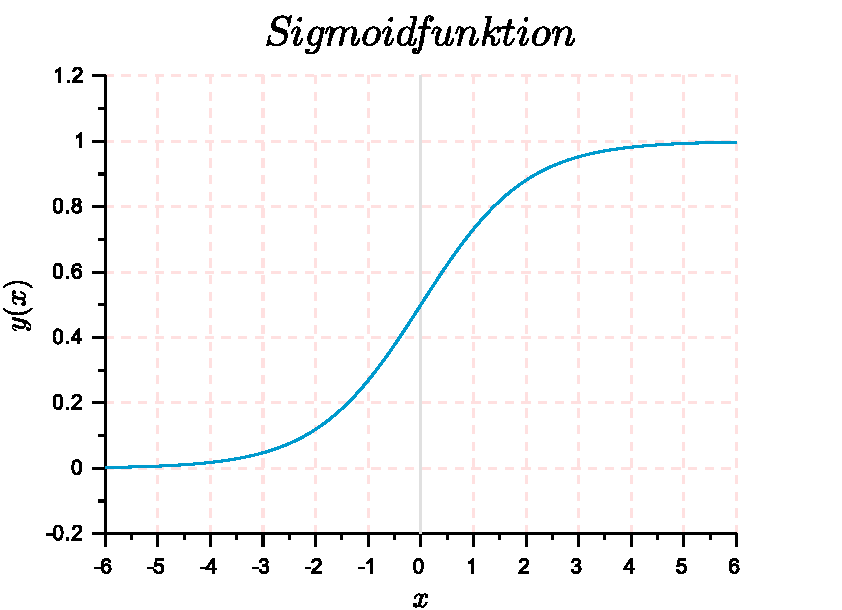
\includegraphics[width=0.3425\textwidth]{images/sigmoid_function}}
% \subcaptionbox{Tangens Hyperbolicus\\$y(x) = tanh(x)$\label{img.tanh_function}}
% {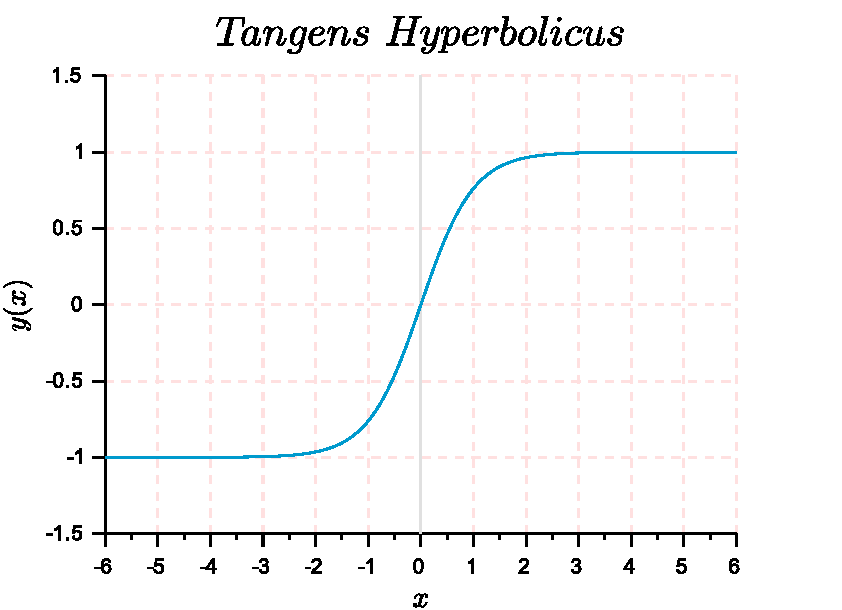
\includegraphics[width=0.3425\textwidth]{images/tanh_function}}
% \subcaptionbox{Maximumsfunktion\\$y(x) = max(0,x)$\label{img.max_function}}
% {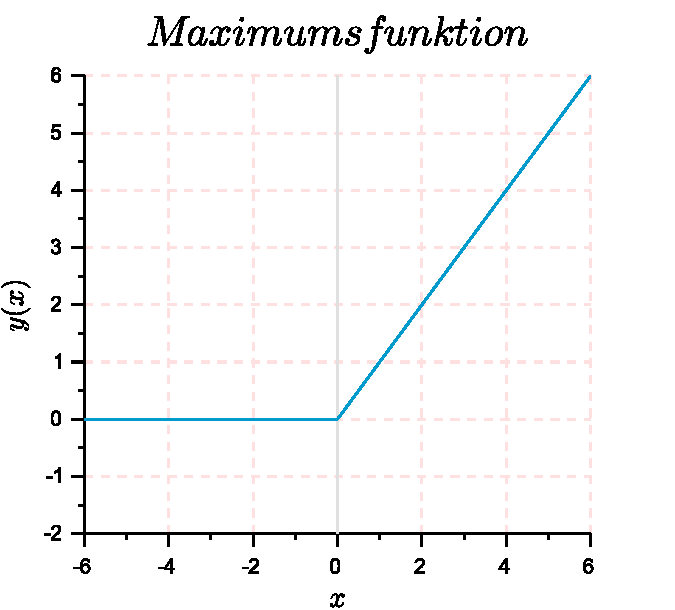
\includegraphics[width=0.275\textwidth]{images/max_function}}
% \caption[Aktivierungsfunktionen eines Neurons]{Mögliche Aktivierungsfunktionen eines Neurons}\label{img.activatefunctions}
% \end{figure}

% Das neuronale Netzwerk ergibt sich aus verschiedenen Ebenen von Neuronen, welche so miteinander verbunden sind, dass die Ausgabe eines Neurons als Eingabe für ein weiteres Neuron der nächsten Ebene dient (vgl. \autoref{img.neural_net_architecture}). Allgemein gibt es drei Arten von Ebenen: Die Eingabe-Ebene, die verborgene Ebene und die Ausgabe-Ebene. Die verborgene Ebene repräsentiert dabei gelernte nicht-lineare Kombinationen der Merkmale des Eingabe-Vektors, sodass damit jede mögliche Funktion darstellbar ist.

% Findet die Informationsweitergabe, wie in \autoref{img.neural_net_architecture} dargestellt, nur in Verarbeitungsrichtung (vom Eingang zum Ausgang) statt, so spricht man von Feedforward-Netzwerken. Gibt es zusätzlich zur Vorwärtsrichtung auch rückgerichtete (\i{rekurrente}) Verbindungen, so spricht man von Recurrent-Netzwerken. Hier ist es durch (oft zeitversetzte) Rückkopplung möglich, Informationen aus vorangegangenen Verarbeitungsschritten wieder als Eingabeinformation zu verarbeiten (vgl. \autoref{ss.rnnlm}).

% \bild{neural_net_architecture}{10cm}{Künstliches neuronales Netzwerk mit einer verborgenen Ebene}{Künstliches neuronales Netzwerk Architektur}

% \section{Training von Modellen}\label{s.training}
% Beim Training eines neuronalen Netzwerk-Modells geht es um das Erlernen einer spezifischen Funktion. Diese Funktion stellt im Allgemeinen die Abbildung bestimmter Merkmale aufgrund gegebener Eingabeinformationen dar. In der Regel geschieht dies durch Modifikation der Gewichtungen zwischen einzelnen Neuronen. Die Modifikation wird im Einzelnen von einem Lernalgorithmus bestimmt, welcher die Größe und Richtung der Gewichtsänderung angibt. Lernalgorithmen sind dabei zwei Kategorien zuzuordnen: überwachtes Lernen und unüberwachtes Lernen (vgl. \autoref{s.maschinelleslernen}). Im Folgenden wird ein mögliches Lernverfahren zum Training eines neuronalen Netzwerks erläutert.

% \subsection{Fehlerminimierung: Gradientenabstieg}\label{ss.sgd}
% Zunächst ist der Gradientenabstieg eine Möglichkeit, ausgehend von einem Näherungswert Minimierungsprobleme zu lösen. Dabei ist das Ziel die Minimierung einer bestimmten Zielfunktion, welche sich aus der Summe differenzierbarer Funktionen ergibt.

% Diese Zielfunktion beschreibt im Zusammenhang mit dem Training neuronaler Netzwerke den Fehler der Ausgabe der einzelnen Neuronen in Abhängigkeit ihrer Gewichtungen. Mithilfe des Gradientenabstiegs kann ausgehend von einem Punkt der Oberfläche der Fehlerfunktion durch iterative Gradientenberechnung solange in Richtung des stärksten Abstiegs gegangen werden, bis ein (lokales) Minimum gefunden wurde. Um den stärksten Abstieg in einem gegebenen Punkt möglichst genau berechnen zu können, werden normalerweise alle zur Verfügung stehenden Trainingsdaten in jeden Berechnungsschritt miteinbezogen. Das bedeutet allerdings einen hohen Aufwand der Gradientenberechnung und damit auch einen entsprechend hohen Aufwand beim Modelltraining.

% Um diesen Aufwand zu reduzieren, gibt es das Gradientenverfahren \i{Stochastic Gradient Descent} (SGD). Die Besonderheit von SGD gegenüber anderen Gradientenverfahren ist, dass nicht alle Trainingsdaten komplett in die Gradientenberechnung der Zielfunktion einbezogen werden, sondern nur ein zufällig gewählter Datensatz\footnote{Aus diesem Grund wurde der Name \i{stochastischer} Gradientenabstieg gewählt.} pro Iterationsschritt. Dadurch ist die Gradientenberechnung hier erheblich schneller. Außerdem hat SGD neben stabilerer Konvergenz auch den Vorteil, dass aufgrund seiner stochastischen Natur parallelisiert trainiert werden kann, was die Trainingsdauer zusätzlich deutlich verringert.

% \autoref{img.sgd} zeigt beispielhaft den Gradientenabstieg einer Funktion $J(\Theta_0, \Theta_1)$ mit den Parameter-Funktionen $\Theta_0$ und $\Theta_1$ bis zu einem lokalen Minimum.

% \bild{sgd}{14cm}{Beispielhafter Gradientenabstieg einer durch Veränderung der Parameter-Funktionen $\Theta_0$ und $\Theta_1$ zu minimierenden Funktion $J(\Theta_0, \Theta_1)$ von einem Ausgangspunkt bis zu einem (lokalen) Minimum}{Beispielhafter Gradientenabstieg}

% \subsection{Lernverfahren: Backpropagation}\label{ss.backpropagation}
% Ziel beim Training neuronaler Netzwerke ist es, den Fehler der Ausgabe zu minimieren, welcher sich durch die Gewichtungen der Neuronenverbindungen ergibt. Backpropagation gehört zu den überwachten Lernverfahren und dient der Anpassung dieser Gewichtungen durch inverses Durchlaufen eines neuronalen Netzwerks. Das Schema der Backpropagation ist in \autoref{img.backpropagation} dargestellt.

% \bild{backpropagation}{12cm}{Backpropagation des bestimmten Fehlers zur Anpassung der Gewichte der Neuronenverbindungen}{Backpropagation}

% Zunächst wird ein Eingabe-Vektor am neuronalen Netzwerk angelegt und vorwärts propagiert, sodass ein Ausgabe-Vektor entsteht, der mit dem Ziel-Vektor verglichen werden kann. Aus der quadrierten Differenz ergibt sich der im Netzwerk entstandene Fehler, entsprechend folgender Formel\footnote{Die Formeln und das Prinzip der Backpropagation wurden von Rumelhart et al. erstmals 1986 vorgestellt \citep{Rumelhart1986}.}:
% \begin{equation}
%     E_p = \frac{1}{2}\sum_{n=1}^N \left(t_{pn} - o_{pn}\right)^2  \label{eq.error_function}
% \end{equation}

% Dabei beschreibt \autoref{eq.error_function} den Fehler $E_p$ bezüglich eines einzelnen Eingabe-Vektors $p$ von $N$ vorhandenen Eingabe-Vektoren mithilfe des Zielwertes $t_p$ und des aktuellen Ausgabewertes $o_n$. Der Gesamtfehler ergibt sich daher aus:
% \begin{equation}
%     E = \sum E_p  \label{eq.total_error_function}
% \end{equation}

% Der errechnete Fehler wird nun von der Ausgabe-Ebene zur Eingabe-Ebene hin zurück propagiert, wobei die Gewichtungen der einzelnen Neuronenverbindungen je nach Einfluss auf den Fehler angepasst werden. Möglich ist das mithilfe des Gradientenabstiegs (wie z.B. SGD):
% \begin{equation}
%     \Delta_pw_{ji} = \eta\delta_{pj}i_{pi}  \label{eq.delta_error_function}
% \end{equation}

% Die Änderung der Gewichtung $\Delta_pw_{ji}$ zwischen dem $i$-ten und $j$-ten Neuron mit Schrittweite $\eta$ wird dabei durch eine Verallgemeinerung der Delta-Regel beschrieben, wobei das Fehlersignal von Neuron $j$ durch $\delta_{pj}$ und die Ausgabe von Neuron $i$ durch $i_{pi}$ dargestellt wird (vgl. Rumelhart et al. 1986 \citep{Rumelhart1986}).

% Wird nun nach der Zurückpropagierung des Fehlers und Anpassung der Gewichte der Eingabe-Vektor erneut an das Netzwerk angelegt, so ergibt sich ein Ausgabe-Vektor, welcher dem Zielvektor ähnlicher ist. So ist es mithilfe von Backpropagation möglich, ein neuronales Netzwerk zu trainieren.

% Beim Zurückpropagieren in sehr großen Netzwerken mit zufällig initialisierten Gewichtungen kann die Gradientenzerstreuung problematisch sein. Durch die hohe Anzahl an Ebenen verteilt sich der zurückpropagierte Fehler auf so viele mögliche Fehlerquellen (Gewichtungen), dass diese kaum mehr geändert werden. Dadurch findet in bestimmten Ebenen kein \q{Lernenprozess} mehr statt. Eine Lösung für dieses Problem ist, die Gewichtungen durch ein unüberwachtes Pre-Training einzelner Ebenen zu initialisieren (Bengio et al. 2007 \citep{Bengio2007}).

% \section{Modelle und Architekturen}\label{s.modelle}
% Mikolov et al., 2013 \cite{Mikolov2013} erläutert verschiedene Modell-Architekturen basierend auf neuronalen Netzwerken wie Feedforward-Netzwerke (vgl. \autoref{ss.nnlm}) und Recurrent-Netzwerke (vgl. \autoref{ss.rnnlm}). Diese repräsentieren Eingabedaten zwar sehr genau, weisen aber für eine große Menge an Trainingsdaten sehr lange Berechnungszeiten auf. Als Hauptursache für den sich ergebenden Aufwand benennen Mikolov et al. die nichtlineare verborgene Ebene der Modelle. Um den Aufwand der Berechnung während des Trainings zu minimieren, wurden zwei vereinfachte\footnote{Die Vereinfachung besteht hier im Weglassen der verborgenen Ebene(n) aus dem neuronalen Netzwerk Modell, welche den Hauptteil der Trainingskomplexität ausmacht.} Modell-Architekturen zum Erlernen von Wort-Vektoren vorgestellt: Continuous-Bag-of-Words (CBOW) und Skip-Gram. Diese Architekturen repräsentieren die Eingabedaten zwar weniger präzise, dafür ermöglichen sie aber eine effizientere Verarbeitung der Trainingsdaten und damit die Verarbeitung größerer, webbasierter Korpora. In den folgenden Unterabschnitten werden die eben genannten Modell-Architekturen nach Mikolov et al., 2013 \cite{Mikolov2013} vorgestellt, basierend auf Bengio et al., 2003 \citep{Bengio2003} und Mikolov et al., 2010 \citep{Mikolov2010}.

% \subsection{Feedforward-Netzwerk Modell}\label{ss.nnlm}
% Das \i{Feedforward Neural Net Language Model} (NNLM) besteht aus Eingabe-Ebene, Projektionsebene, verborgener Ebene und Ausgabe-Ebene, welche nur in eine Richtung von der Eingabe- zur Ausgabe-Ebene miteinander verbunden sind (vgl. \autoref{img.neural_net_architecture}). In der Eingabe-Ebene werden $N$ vorangehende Wörter One-Hot-kodiert, sodass sie die Größe $V$ des Vokabulars aufweisen. Anschließend findet mithilfe einer gemeinsamen Projektionsmatrix eine Projektion von der Eingabe-Ebene zur Projektionsebene mit der Dimension $N \times D$ statt, wobei $D$ die Größe der Merkmalsvektoren bezeichnet. Die verborgene Ebene mit der Dimension $H$ dient hierbei der Berechnung der Wahrscheinlichkeitsverteilung über alle Wörter des Vokabulars, sodass die Ausgabe-Ebene die Dimension $V$ aufweist. Mikolov et al. geben folgenden Aufwand des Trainings an:
% \begin{equation}
%     Q = N \times D + N \times D \times H + H \times V \label{eq.complexitiy_nnlm}
% \end{equation}

% Der Aufwand des dominierenden Terms $H \times V$ kann durch Trainingsoptimierungen wie z.B. Hierarchical Softmax (vgl. \autoref{ss.hierarchical_softmax}) auf $H \times \log_2(V)$ reduziert werden, da in diesem Fall das Vokabular als Binärbaum modelliert wird. Weiterhin wird der Gesamtaufwand von dem Term $N \times D \times H$ bestimmt. Hier ist ersichtlich, dass der Aufwand von der Dimension der verborgenen Ebene $H$ abhängt.

% \subsection{Recurrent-Netzwerk Modell}\label{ss.rnnlm}
% Das \i{Recurrent Neural Net Language Model} (RNNLM) wurde als Verbesserung des NNLM vorgestellt, da RNNLM nach Mikolov et al. in der Theorie komplexere Muster effizienter repräsentieren können. Das RNNLM besteht aus Eingabe-Ebene, verborgener Ebene und Ausgabe-Ebene. Statt einer Projektionsebene verfügt die verborgene Ebene hier über zeitverzögernde Verbindungen (vgl. \autoref{img.recurrent_neural_net_architecture}). Dadurch können Informationen aus vorangegangenen Zeitschritten in das aktuelle Training miteinbezogen werden. Mikolov et al. geben folgenden Aufwand des Trainings an:
% \begin{equation}
%     Q = H \times H + H \times V \label{eq.complexitiy_rnnlm}
% \end{equation}

% Wie beim Feedforward-Netzwerk kann auch hier $H \times V$ zu $H \times \log_2(V)$ durch Binärbaum-Repräsentation des Vokabulars optimiert werden, wodurch der Aufwand maßgeblich von $H \times H$, also erneut der Dimension der verborgenen Ebene, bestimmt wird.

% \bild{recurrent_neural_net_architecture}{10cm}{Architektur des Recurrent-Netzwerk Modell}{Architektur des Recurrent-Netzwerk Modell mit rückgerichteten Kanten}

% \subsection{Continuous-Bag-of-Words Architektur}\label{ss.cbow}
% Ziel der CBOW Architektur ist es, die Vektor-Repräsentation eines Wortes mit geringerem Aufwand als NNLM und RNNLM zu ermitteln. Die Merkmale eines Wortes sollen hier nicht mehr mithilfe verborgener Ebenen des neuronalen Netzwerks, sondern durch den Kontext repräsentiert werden, in dem das Wort steht. Die Architektur ist in \autoref{img.cbow_architecture} dargestellt.

% \bild{cbow_architecture}{15cm}{CBOW-Architektur mit einer Fenstergröße von 2: Lernen des Wort-Vektors zum Wort \q{hat} anhand eines Beispielkontextes.}{CBOW-Architektur}

% Der Kontext wird durch ein Eingabe-Fenster beschrieben, dessen Breite die Wortanzahl vor und hinter dem Zielwort vorgibt. Die Vektoren der Kontext-Wörter ergeben sich initial aus einer einfachen Repräsentation (wie beispielsweise die One-Hot Kodierung, vgl. \autoref{ss.onehot}) und werden in der Projektionsebene zu einem Vektor vereint (z.B. durch Summen- oder Durchschnittsbildung), welcher anschließend als Eingabe für ein neuronales Netzwerk ohne verborgene Ebene dient. In diesem Modell werden die Gewichte der Neuronenverbindungen trainiert, indem auf den entstehenden Vektor die Aktivierungsfunktion angewendet wird. Anhand des Ergebnisses kann entschieden werden, ob dieser das Zielwort repräsentiert. Falls dies nicht der Fall ist, werden die Gewichte durch Backpropagation (vgl. \autoref{ss.backpropagation}) angepasst. Mit dieser Architektur ist demnach ein unüberwachtes Lernen möglich, indem Wörter durch ihren Kontext beschrieben werden.


% Durch den Entfall einer verborgenen Ebene ergibt sich nach Mikolov et al. für das CBOW Modell der in \autoref{eq.complexitiy_cbow} dargestellte Aufwand, welcher deutlich geringer ist als bei NNLM oder RNNLM.
% \begin{equation}
%     Q = N \times D + N \times \log_2(V) \label{eq.complexitiy_cbow}
% \end{equation}


% \subsection{Skip-Gram Architektur}\label{ss.skipgram}
% Wie bereits bei CBOW nutzt die Skip-Gram Architektur die Tatsache aus, dass im Normalfall dicht beieinander stehende Wörter eher miteinander korrelieren als weit von einander entfernte. Anders als CBOW sucht Skip-Gram allerdings Vektor-Repräsentationen von Wörtern, welche dazu geeignet sind, die Wörter im jeweiligen Kontext vorherzusagen. Dazu dient jedes Wort als Eingabe eines log-linearen Klassifizierers, welcher in der Projektionsebene die Wahrscheinlichkeiten der vorhergehenden und nachfolgenden Wörter errechnet. \autoref{eq.average_log_probability} stellt die durchschnittliche logarithmische Wahrscheinlichkeit für eine Folge von Trainingsworten $w_1, w_2, \cdots, w_T$ dar, welche Skip-Gram maximieren möchten:

% \begin{equation}
%     \frac{1}{T}\sum_{t=1}^T\sum_{-C\leq j \leq C} \log p\left(w_{t+j}|w_t\right), j \neq 0  \label{eq.average_log_probability}
% \end{equation}

% Dabei bezeichnet $C$ die Anzahl von Wörtern vor und nach dem gegebenen Wort $w_t$ (Fensterbreite). Mikolov et al. haben gezeigt, dass größere $C$ zwar mehr Trainings-Beispiele liefern und folglich zu höherer Genauigkeit der Wort-Vektoren führen können, allerdings auf Kosten von Rechenkomplexität und Trainingszeit.

% Der Aufwand des Trainierens mittels Skip-Gram wird von Mikolov et al. wie folgt angegeben:
% \begin{equation}
%     Q = C \times (D + D \times \log_2(V)) \label{eq.complexitiy_skipgram}
% \end{equation}

% \section{Optimierungen}\label{ss.modellverbesserungen}
% Im Folgenden werden Methoden zur Optimierung des Rechenaufwands des Trainings und der Verbesserung trainierter Sprachmodelle vorgestellt.

% \subsection{Hierarchical Softmax}\label{ss.hierarchical_softmax}
% Für Modelle basierend auf neuronalen Netzwerken muss die bedingte Wahrscheinlichkeit aller Wörter aus dem Vokabular aufgrund eines gegebenen Kontextes berechnet werden. Anschließend wird eine Normalisierung (engl. \i{Softmax}) durchgeführt, um den Einfluss von Extremwerten oder Ausreißern zu vermindern, ohne diese zu entfernen. Diese Operationen sind sehr rechenaufwändig, da sie das gesamte Vokabular betreffen.

% Hierarchical Softmax wurde in seinem Grundkonzept 2005 von F. Morin und Y. Bengio vorgestellt \citep{Morin2005}\footnote{Die Ausführungen in diesem Abschnitt beziehen sich jedoch auf einen wissenschaftlichen Artikel von Xin Rong \citep{Rong}.} und stellt eine recheneffiziente Möglichkeit der Berechnung einer solchen Normalisierung dar. Hier werden alle Wörter des Vokabulars als Blätter eines Binärbaums repräsentiert, welcher mittels Huffman-Kodierung\footnote{Von David A. Huffman 1952 entwickelte Kodierungsform, bei welcher jedem Element ein Codewort variabler Länge zugeordnet wird, um dieses möglichst redundanzfrei abzubilden.} konstruiert wird. Basierend auf der jeweiligen Worthäufigkeit besitzt jede Verbindung zweier Knoten eine bestimmte Wahrscheinlichkeit. Für jedes Wort existiert jetzt genau ein Pfad von der Wurzel zum Blatt, welcher genutzt werden kann, um die Wahrscheinlichkeit eines Wortes durch Multiplikation der Teil-Wahrscheinlichkeiten zu schätzen. Somit wird der Aufwand des Trainings von $O(V)$ auf $O(\log(V))$ reduziert, wobei $V$ die Anzahl der Wörter im Vokabular bezeichnet.

% In \autoref{img.hierarchical_softmax} ist die Berechnung der Wahrscheinlichkeit beispielhaft für ein Wort $w_2$ dargestellt. Der Pfad zu $w_2$ besteht aus 3 Kanten von der Wurzel $n_0$ über die Knoten $n_1$ und $n_3$, für welche jeweils die Wahrscheinlichkeit in Abhängigkeit vorheriger Kanten berechnet werden kann. Dabei bezeichnet $p_{n_k}$ die Wahrscheinlichkeit des $k$-ten Knotens, $p_{w_i}$ die Wahrscheinlichkeit des $i$-ten Wortes und $P_{L,n_k}$ die Wahrscheinlichkeit, dass das Wort ausgehend vom Knoten $n_k$ links liegt.

% \bild{hierarchical_softmax}{14cm}{Hierarchical Softmax: Huffmann-Binärbaum mit einem Beispielpfad für die Wahrscheinlichkeitsberechnung von Wort $w_2$ eines Vokabulars der Größe $V$.}{Hierarchical Softmax}


% \subsection{Negative Sampling}\label{ss.negative_sampling}
% Neben Hierarchical Softmax ist Negative Sampling eine Möglichkeit der Qualitätsverbesserung trainierter Modelle. Nach Mikolov et al. \citep{Mikolov2013Dist} dient Negative Sampling der Modellverbesserung, indem nicht nur korrekte Fälle aus den Trainingsdaten, sondern auch bewusst nicht in den Trainingsdaten vorkommende, falsche Beispiele (\i{negative samples}) generiert und beim Training mit einbezogen werden\footnote{Da in dieser Arbeit Sprachmodelle auf Textkorpora trainiert werden, sind \q{negative samples} hier zufällig aus dem Vokabular gewählte Wörter.}. Diese Art von künstlicher Varianz beim Training sorgt dafür, dass mit Negative Sampling trainierte Modelle weniger fehleranfällig sind und somit bessere Evaluierungsergebnisse liefern. Der modellverbessernde Effekt von Negative Sampling hängt dabei stark von der Anzahl der jeweils verwendeten Negative Samples ab.

% % ==================================================================================================
% \chapter{Methodik und Implementierung}\label{c.implementierung}
% Nachdem in den vorangegangen Kapiteln die theoretische Grundlage für die Methodik und Umsetzung in NLP allgemein und für diese Arbeit im einzelnen gelegt wurde, präsentiert dieses Kapitel die speziell für diese Arbeit entwickelte und verwendete Methodik. Dies beinhaltet die praktische Umsetzung des Trainierens deutscher Wort-Vekoren: den Bezug und die Erstellung von Korpora und den Aufbau eines Toolkits zum Training und anschließender Evaluierung.

% \section{Erstellung des Korpus}\label{s.korpuserstellung}
% Zum Trainieren von Sprachmodellen sind große Mengen von Trainingsdaten in Textform notwendig. Da es in dieser Arbeit um die Analyse deutscher Sprachmodelle geht, werden deutsche Texte benötigt, welche thematisch vielfältig, dabei jedoch nicht umgangssprachlich sind.

% Eine Möglichkeit zum Bezug öffentlicher deutscher Trainingsdaten ist die deutsche Wikipedia. Mit über 1,8 Millionen Artikeln\footnote{Offizielle Wikipedia-Statistik zur Artikelanzahl (o.J.), URL: \url{http://stats.wikimedia.org/DE/TablesArticlesTotal.htm} (Stand: 08.05.2015)} stellt die deutsche Wikipedia eine große Anzahl von Wörtern in natürlicher deutscher Sprache zur Verfügung. Artikelinhalte können per Wikipedia Datenbank Backup Dump\footnote{Dateiliste deutscher Wikipedia Dumps (o.J.), URL: \url{http://dumps.wikimedia.org/dewiki/latest/} (Stand: 08.05.2015)} bezogen werden. Dieser Dump besteht aus einer komprimierten XML-Datei, welche die Artikel jeweils als einzelne XML-Objekte enthält. Ein solches XML-Objekt besteht neben dem eigentlichen Artikelinhalt auch aus Metainformationen wie Titel, Zeitstempel und Autor. Außerdem ist der Artikelinhalt in MediaWiki Markup\footnote{Formatierungen mittels MediaWiki Markup (o.J.), URL: \url{http://www.mediawiki.org/wiki/Help:Formatting}} notiert, um Textformatierungen und das Einfügen von Tabellen, Formeln, Bildern und HTML zu ermöglichen. Für das Modelltraining müssen die Trainingsdaten in reiner Textform vorliegen, da andernfalls die durch die Notation verfälschten Wörter gelernt werden. Aus diesem Grund müssen sowohl die XML-Tags als auch das MediaWiki Markup entfernt werden. Der \i{Wikipedia Extractor} ist ein von Giuseppe Attardi (Universität von Pisa) geschriebenes freies Python Script\footnote{Dokumentation und Download des \i{Wikipedia Extractor} unter GPL3 Lizenz (o.J.), URL: \url{http://medialab.di.unipi.it/wiki/Wikipedia_Extractor}}, das die beschriebene Filterung des Wikipedia Dumps bewerkstelligt.

% Außerdem gibt es eine zum Buch \q{Statistical Machine Translation} von Philipp Koehn gleichnamige Website\footnote{Koehn, Philipp: Statistical Machine Translation (o.J.), URL: \url{http://www.statmt.org/} (Stand: 08.05.2015)}, auf welcher für die automatisierte Übersetzung von Texten öffentliche Trainingsdaten in Form von einsprachigen Nachrichtenartikeln zur Verfügung gestellt werden. Diese sind jahrweise komprimiert und für die deutsche Sprache von 2007 bis 2013 vorhanden\footnote{Dateiliste verschiedensprachiger Nachrichtenartikel aus den Jahren 2007 bis 2013 (o.J.), URL: \url{http://www.statmt.org/wmt14/training-monolingual-news-crawl/} (Stand: 08.05.2015)}.

% % Es gibt weitere mögliche öffentliche Korpora, wie beispielsweise den deutschen Referenzkorpus (DeReKo\footnote{Gepflegt vom Institut für Deutsche Sprache. IDS: Korpuslinguistik (o.J), URL: \url{http://www1.ids-mannheim.de/kl/projekte/korpora.html} (Stand: 07.07.2015)})

% In dieser Arbeit wird entsprechend der Trainingsumgebung (vgl. \autoref{ss.trainingsumgebung}) der Korpus für die Modellierung aus dem Wikipedia Dump der deutschen Wikipedia und deutschen Nachrichtenartikeln aus dem Jahr 2013 bestehen. Dieser Korpus enthält insgesamt über 1,1 Milliarden Wörter in knapp 60 Millionen Sätzen und ist 7,49 GB groß. %Dieser Korpus enthält insgesamt 1.111.394.783 Wörter in 59.670.477 Sätzen und ist 7,49 GB groß.

% In \autoref{tab.corpus} sind die einzelnen statistischen Daten der Teilkorpora aufgelistet. Das Erkennen von Sätzen und Wörtern (Tokenisierung) wird im folgenden Abschnitt erläutert.

% \begin{table}[!ht]\vspace{1ex}\small\centering\def\arraystretch{1.1}\begin{tabular}{|l|c|c|c|c|}
% \hline Korpus & Wortanzahl & Satzanzahl & Vokabulargröße & Korpusgröße \\ \hline\hline
% Wikipedia & \tt{ \ 579.046.421} & \tt{24.656.073} & \tt{14.418.176} & \tt{3,95 GB} \\ \hline
% Nachrichten & \tt{ \ 532.348.362} & \tt{35.014.404} & \tt{\ 9.256.424} & \tt{3,54 GB} \\ \hline\hline
% Gesamt & \tt{1.111.394.783} & \tt{59.670.477} & \tt{20.705.362} & \tt{7,49 GB} \\ \hline
% \end{tabular}
% \caption[Korpus Statistik]{\label{tab.corpus}Korpus Statistik des deutschen Wikipedia Dumps 2015 und deutscher Nachrichtenartikel von 2013.}
% \vspace{1ex}\end{table}


% \section{Korpus Preprocessing}\label{s.preprocessing}
% Beim Preprocessing wird der Korpus für das Training vorbereitet und bearbeitet, um bei der Evaluation der trainierten Sprachmodelle festzustellen, ob diese verbessert wurden oder nicht. Mithilfe des \i{Natural Language Toolkit} (NLTK\footnote{NLTK ist eine Sammlung von Bibliotheken und Programmen in Python zur Verarbeitung natürlicher Sprache wie Klassifizierung, Tokenisierung und Tagging. Natural Language Toolkit (o.J.), URL: \url{http://www.nltk.org}}) werden die durch den Korpus zur Verfügung stehenden Textdaten in einzelne Sätze und diese wiederum in einzelne Wort-Tokens zerlegt. Diese Tokenisierung geschieht mit der \tt{word\_tokenize()}-Funktion von NLTK, basierend auf einem für deutsche Tokenisierung vortrainierten Modell\footnote{Dieses Modell wurde auf der Neuen Züricher Zeitung trainiert und enthält 847k Tokens. Text Mining online (o.J.), URL: \url{http://textminingonline.com/tag/nltk-word-tokenize} (Stand: 29.06.2015)}.

% Anschließend ist es möglich, einzelne Tokens auszuschließen bzw. zu normalisieren, um Aussagen darüber treffen zu können, ob derartiges Preprocessing Sprachmodelle verbessern kann.

% Zunächst kann die Interpunktion entfernt werden. Dazu steht die folgende im DIMA-Projekt (Arras et al. \citep{Arras2014}) verwendete Zeichenliste zur Verfügung:

% \code{. .. ... , ; : ( ) " \ \lq \ [ ] \{ \} ? ! - — + * {-}- `` ''}

% Neben der Interpunktion können auch Stoppwörter entfernt werden. Stoppwörter sind Wörter, welche sehr oft im Korpus auftreten, dabei aber kaum einen inhaltlichen Mehrwert bieten. Deutsche Stoppwörter sind z.B. bestimmte Artikel (\q{der}, \q{die}, \q{das}) oder Konjunktionen (\q{und}, \q{oder}). \autoref{lst.stopwords} zeigt die in dieser Arbeit verwendete Liste deutscher Standard-Stoppwörter von NLTK.

% Darüber hinaus ist eine Normalisierung des Korpus bezüglich deutscher Umlaute und \sq{ß} möglich. Dazu werden die Umlaute in ihre entsprechende Digraph-Repräsentation umgewandelt (ä $\rightarrow$ ae,\ "s $\rightarrow$ ss \ etc.). Diese Normalisierung stellt sicher, dass die Umlaute im Korpus einheitlich dargestellt werden und wurde in das Preprocessing in dieser Arbeit mit einbezogen.

% Schließlich können Bigramme gebildet werden. Bigramme sind Tokens, bestehend aus zwei Wort-Tokens, welche häufig gemeinsam (hintereinander) auftreten (z.B. \q{Angela}, \q{Merkel} $\rightarrow$ \q{Angela\_Merkel}). Semantische Zusammenhänge sollen dadurch deutlich besser dargestellt werden können. Nach Mikolov et al. \citep{Mikolov2013Dist} werden Bigramme aufgrund der Anzahlen der beiden einzelnen Wörter $w_i$ und $w_j$ und deren gemeinsamen Vorkommen $w_iw_j$ nach folgender Formel gebildet (das $\delta$ ist dabei ein Koeffizient zur Vermeidung von Bigrammen zu selten auftretender Wörter):

% \begin{equation}
%     score(w_i,w_j) = \frac{count(w_iw_j)-\delta}{count(w_i)\times count(w_j)} \label{eq.bigram}
% \end{equation}

% Das Ergebnis $score(w_i,w_j)$ wird dabei größer, je öfter zwei Wörter gemeinsam und je seltener beide Wörter einzeln auftreten. Dadurch werden die Wörter \q{Angela Merkel} zu einem Bigram, die Wörter \q{das ist} aber nicht. Liegt das Ergebnis über einem zuvor festgelegtem Schwellenwert, so werden beide Wörter zu einem Bigramm verbunden. In dieser Arbeit wird dafür der Standardwert der Implementierung von NLTK verwendet.

% \autoref{tab.preprocessingstats} zeigt einige Statistiken zu den einzelnen Schritten des Preprocessing.

% \begin{table}[!ht]\vspace{1ex}\small\centering\def\arraystretch{1.1}\begin{tabular}{|l|c|c|c|}
% \hline Preprocessing & Wortanzahl & Vokabulargröße & Datenmenge \\ \hline\hline
% \tt{RAW}  & \tt{1.111.394.783}  & \tt{20.705.362} & 7,49 GB \\ \hline
% \tt{PS}   & \tt{ \ 702.510.144} & \tt{13.197.231} & 5,65 GB \\ \hline
% \tt{PSU}  & \tt{ \ 714.311.955} & \tt{13.160.241} & 5,72 GB \\ \hline
% \tt{PSUB} & \tt{ \ 651.219.519} & \tt{13.757.051} & 5,69 GB \\ \hline
% \end{tabular}
% \caption[Korpus Preprocessing Statistiken]{\label{tab.preprocessingstats}Statistiken zum Korpus Preprocessing\\\tt{RAW } = kein Preprocessing\\\tt{PS \ } = Interpunktions-, Stoppwortfilterung\\\tt{PSU } = Interpunktions-, Stoppwortfilterung, Umlaut-Normalisierung\\\tt{PSUB} = Interpunktions-, Stoppwortfilterung, Umlaut-Normalisierung, Bigramme}
% \vspace{1ex}\end{table}
% % Satzanzahl
% % 59.670.477
% % 72.449.746
% % 72.454.876
% % 72.454.876

% \section{Modell Training}\label{s.modelltraining}
% Um Modelle auf natürlicher Sprache zu trainieren, werden in dieser Arbeit verschiedene Methoden gezeigt. Insbesondere CBOW und Skip-Gram sind Beispiele für Architekturen, die auf neuronalen Netzwerken ohne verborgene Ebene basieren, um die Rechenkomplexität zu reduzieren und die Menge verarbeitbarer Trainingsdaten zu vergrößern. Das dafür im Rahmen dieser Arbeit entwickelte Toolkit und eine bereits existierende Implementierung dieser beiden Architekturen wird im Folgenden beschrieben und später für das Modelltraining und die anschließende Evaluation verwendet.

% \subsection{Software Toolkit}\label{ss.softwaretoolkit}
% Das für Forschungszwecke frei verfügbares Open Source Projekt \i{word2vec} ist ein auf der Arbeit von Mikolov et. al \citep{Mikolov2013} basierendes Software Tool. Es stellt eine effiziente Implementierung der CBOW und Skip-Gram Architektur in C dar\footnote{word2vec Tool (o.J.), URL: \url{https://code.google.com/p/word2vec/} (Stand: 22.06.2015)}. Darauf aufbauend wurden die Trainingsalgorithmen von \i{word2vec} nach Python übertragen, in die Python Bibliothek \i{gensim} aufgenommen und mit zusätzlichen Funktionalitäten (wie z.B. Funktionen zum Vergleich der Wort-Vektoren und Bewertung der Modellgenauigkeit) erweitert\footnote{Rehurek, Radim: Deep learning with word2vec (o.J.), URL: \url{https://radimrehurek.com/gensim/models/word2vec.html} (Stand: 22.06.2015)}. Aufgrund dieser Zusatzfunktionen und der Geschwindigkeitsoptimierungen\footnote{Rehurek, Radim: Machine Learning Blog. (o.J.), URL: \url{http://radimrehurek.com/2013/09/word2vec-in-python-part-two-optimizing/} (Stand: 22.06.2015)} beim Training mit \i{gensim}, wird das Tool zum Modelltraining in dieser Arbeit verwendet.

% \subsection{Mögliche Parameterkonfiguration}\label{ss.parameter}
% Beim Trainieren mit \i{gensim} können die im Folgenden beschriebenen Parameter konfiguriert werden\footnote{In Klammern stehen jeweils die in \autoref{tab.parameter} zur Parameter-Spezifikation verwendeten Kürzel.}.

% Als \b{Modell Architektur (A)} kann für das Modelltraining entweder Skip-Gram oder CBOW verwendet werden. Dabei verfügbare Optimierungen sind \b{Hierarchical Softmax (HS)} und \b{Negative Sampling (NS)}, wobei für
% Negative Sampling die Anzahl der \q{künstlichen Wörter} (engl. \i{negative samples}) spezifiziert werden kann. Die \b{Vektorgröße (D)} bezeichnet die Dimension der Wort-Vektoren, die \b{Fensterbreite (N)} ist der Maximalabstand des aktuellen Wortes zum vorhergesagten Wort innerhalb eines Satzes. Ein Wort wird nur dann in das Training mit einbezogen, wenn es mindestens so häufig wie die von der \b{Worthäufigkeit (R)} festgelegte Mindestanzahl (absoluter Zahlenwert) auftritt. Andernfalls tritt das Wort zu selten auf und wird ignoriert, da in diesem Fall ein zu wenig aussagekräftiger Wort-Vektor entstehen würde. Wird CBOW als Architektur gewählt, so kann die \b{Projektionsart (P)} spezifiziert werden. Diese legt fest, ob aus den Kontext-Vektoren bei der Projektion die Summe oder der Durchschnitt gebildet wird. Die für das parallelisierte Training verwendete \b{Anzahl der Threads} beschleunigt das Training erheblich bei Mehrkern-Prozessoren. Um die Trainingszeit zu minimieren sollte hier die maximale Anzahl der zur Verfügung stehenden Prozessorkerne ausgenutzt werden, in dieser Arbeit 4 (vgl. \autoref{ss.trainingsumgebung}). Das in \autoref{s.preprocessing} beschriebene \b{Preprocessing (P)} beinhaltet die Filterung der Interpunktion \tt{P} und Stoppwörter \tt{S}, die Umwandlung der Umlaute in ihre entsprechende Digraph-Repräsentation \tt{U} oder das zusätzliche Bilden von Bigrammen \tt{B}.

% Durch Kombination der unterschiedlichen Parameter ergeben sich die in \autoref{tab.parameter} dargestellten Parameter-Spezifikationen der trainierten Modelle, unterteil in 8 Evaluationsgruppen.

% \begin{table}[!ht]\vspace{1ex}\small\centering\def\arraystretch{1.0}\begin{tabular}{|l|l|l|c|c|c|c|c|c|}
% \hline Modellname & A         & Pr         & D   & N  & HS   & NS   & R  & P \\ \hline\hline
% \tt{SG-52-5-133M} & Skip-Gram & ---        & 52  & 5  & Ja   & Nein & 5  & ---    \\ \hline
% \tt{SG-52-5-266M} & Skip-Gram & ---        & 52  & 5  & Ja   & Nein & 5  & ---    \\ \hline
% \tt{SG-52-5-530M} & Skip-Gram & ---        & 52  & 5  & Ja   & Nein & 5  & ---    \\ \hline
% \tt{SG-52-5-1B}   & Skip-Gram & ---        & 52  & 5  & Ja   & Nein & 5  & ---    \\ \hline\hline
% \tt{SG-52-5-RAW}  & Skip-Gram & ---        & 52  & 5  & Ja   & Nein & 5  & ---    \\ \hline
% \tt{SG-52-5-PS}   & Skip-Gram & P, S       & 52  & 5  & Ja   & Nein & 5  & ---    \\ \hline
% \tt{SG-52-5-PSU}  & Skip-Gram & P, S, U    & 52  & 5  & Ja   & Nein & 5  & ---    \\ \hline
% \tt{SG-52-5-PSUB} & Skip-Gram & P, S, U, B & 52  & 5  & Ja   & Nein & 5  & ---    \\ \hline\hline
% \tt{SG-52-5}      & Skip-Gram & P, S, U, B & 52  & 5  & Ja   & Nein & 5  & ---    \\ \hline
% \tt{SG-52-10}     & Skip-Gram & P, S, U, B & 52  & 10 & Ja   & Nein & 5  & ---    \\ \hline
% \tt{SG-52-15}     & Skip-Gram & P, S, U, B & 52  & 15 & Ja   & Nein & 5  & ---    \\ \hline
% \tt{SG-52-20}     & Skip-Gram & P, S, U, B & 52  & 20 & Ja   & Nein & 5  & ---    \\ \hline\hline
% \tt{SG-52-5-R10}  & Skip-Gram & P, S, U, B & 52  & 5  & Ja   & Nein & 5  & ---    \\ \hline
% \tt{SG-100-5-R10} & Skip-Gram & P, S, U, B & 100 & 5  & Ja   & Nein & 5  & ---    \\ \hline
% \tt{SG-200-5-R10} & Skip-Gram & P, S, U, B & 200 & 5  & Ja   & Nein & 5  & ---    \\ \hline
% \tt{SG-300-5-R10} & Skip-Gram & P, S, U, B & 300 & 5  & Ja   & Nein & 5  & ---    \\ \hline\hline
% \tt{CB-52-5}      & CBOW      & P, S, U, B & 52  & 5  & Ja   & Nein & 5  & $\sum$ \\ \hline
% \tt{CB-52-10}     & CBOW      & P, S, U, B & 52  & 10 & Ja   & Nein & 5  & $\sum$ \\ \hline
% \tt{CB-52-15}     & CBOW      & P, S, U, B & 52  & 15 & Ja   & Nein & 5  & $\sum$ \\ \hline
% \tt{CB-52-20}     & CBOW      & P, S, U, B & 52  & 20 & Ja   & Nein & 5  & $\sum$ \\ \hline\hline
% \tt{SG-52-5}      & Skip-Gram & P, S, U, B & 52  & 5  & Ja   & Nein & 5  & ---    \\ \hline
% \tt{SG-52-5-NS10} & Skip-Gram & P, S, U, B & 52  & 5  & Ja   & 10   & 5  & ---    \\ \hline
% \tt{SG-52-5-NS20} & Skip-Gram & P, S, U, B & 52  & 5  & Ja   & 20   & 5  & ---    \\ \hline
% \tt{SG-52-5-NS30} & Skip-Gram & P, S, U, B & 52  & 5  & Ja   & 30   & 5  & ---    \\ \hline\hline
% \tt{SG-52-5}      & Skip-Gram & P, S, U, B & 52  & 5  & Ja   & Nein & 5  & ---    \\ \hline
% \tt{SG-52-5-R10}  & Skip-Gram & P, S, U, B & 52  & 5  & Ja   & Nein & 10 & ---    \\ \hline
% \tt{SG-52-5-R20}  & Skip-Gram & P, S, U, B & 52  & 5  & Ja   & Nein & 20 & ---    \\ \hline
% \tt{SG-52-5-R50}  & Skip-Gram & P, S, U, B & 52  & 5  & Ja   & Nein & 50 & ---    \\ \hline\hline
% \tt{CB-52-5-SUM}  & CBOW      & P, S, U, B & 52  & 5  & Ja   & Nein & 5  & $\sum$ \\ \hline
% \tt{CB-52-5-MEAN} & CBOW      & P, S, U, B & 52  & 5  & Ja   & Nein & 5  & \O     \\ \hline
% \tt{SG-52-5-HS}   & Skip-Gram & P, S, U, B & 52  & 5  & Ja   & Nein & 5  & ---    \\ \hline
% \tt{SG-52-5-NOHS} & Skip-Gram & P, S, U, B & 52  & 5  & Nein & Nein & 5  & ---    \\ \hline
% \end{tabular}
% \caption[Parameter-Spezifikationen trainierter Modelle]{\label{tab.parameter}Parameter-Spezifikationen trainierter Modelle zur Architektur $A$, Preprocessing $Pr$, Vektordimension $D$, Fensterbreite $N$, Hierarchical Softmax $HS$, Negative Sampling $NS$, Worthäufigkeit $R$ und Projektionsart $P$}
% \vspace{1ex}\end{table}


% \subsection{Trainingsumgebung}\label{ss.trainingsumgebung}
% Alle Modelle wurden auf einem Desktop-Rechner unter Ubuntu 14.04 mit 16 GB RAM trainiert. Dabei kam eine 4-Kern AMD A10-7850K Radeon R7 CPU zum Einsatz, welche mit 3.7 GHz taktet. Korpora und Modell wurden dabei auf einer SSD-Festplatte gespeichert. %Diese Trainingsumgebung entspricht damit der Spezifikation eines Rechners für den normalen Heimgebrauch.

% \section{Evaluation der Wort-Vektoren}\label{s.evaluation}
% Um die trainierten Modelle miteinander vergleichen zu können, ist es notwendig, diese mithilfe geeigneter Test-Sets zu evaluieren. Anhand der Testergebnisse kann anschließend entschieden werden, welches Modell und damit welche Parameter-Konfiguration die besten Wort-Vektoren erzeugt hat.

% Angelehnt an Mikolov et al. \citep{Mikolov2012} werden in dieser Arbeit die Modelle durch Test-Sets mit Analogiefragen der Form \q{\tt{a} verhält sich zu \tt{b}, wie \tt{c} zu \tt{d}} zum einen zur Syntax und zum anderen zur Semantik evaluiert\footnote{Zu beachten ist dabei, dass die Modelle zur Nutzung großer Korpora unüberwacht trainiert wurden, sodass diese Fragen nicht Teil des Trainings waren.}. Praktisch bedeuten Analogiefragen das Ausführen einer Vektoraddition der entsprechenden Wort-Vektoren, z.B.:\\
% \tt{vector(K"onig) - vector(Mann) + vector(Frau) $\approx$ vector(K"onigin)}\\
% Dabei ergibt sich aus der linken Seite der Gleichung ein Vektor, für welchen mithilfe der Kosinusähnlichkeit geprüft werden kann, welcher Vektor der Ähnlichste im Umfeld ist. Dieser stellt dann die Antwort der Analogiefrage dar. Ist es der Vektor des in der Frage angegebenen Wortes (im Beispiel der Vektor des Wortes \q{Königin}), so wurde die Frage korrekt beantwortet. Lag der Ziel-Vektor unter den 10 ähnlichsten Vektoren, so war die korrekte Antwort auf die Frage unter den Top 10 Ergebnissen.

% Teil dieser Arbeit ist die Erstellung entsprechender deutscher Test-Sets, welche online zum freien Download zur Verfügung stehen\footnote{Müller, Andreas: GermanWordEmbeddings (o.J.), URL: \url{http://devmount.github.io/GermanWordEmbeddings} (Stand: 22.06.2015)}. Die Fragen der erstellten Test-Sets enthalten dabei keine Bigramm-Tokens, um auch Modelle, welche keine Bigramm-Tokens enthalten, mit den gleichen Fragen evaluieren zu können.

% \subsection{Syntaktisches Test-Set}\label{ss.syntactictestset}
% Um syntaktische Zusammenhänge in der deutschen Sprache abfragen zu können, werden Analogiefragen zu unterschiedlichen Formen von Nomen, Adjektiven und Verben verwendet. Dazu wird eine Liste von jeweils 100 gängigen Wörtern zu jeder der drei Wortarten erstellt\footnote{Gebräuchliche Wörter sind beispielsweise bei Angeboten für Deutsch-Lernende zu finden. Die Wörter der Listen dieser Test-Sets entstammen \i{The German Professor} (o.J.), URL: \url{http://www.thegermanprofessor.com/top-100-german-verbs/} (Stand: 18.05.2015) und \url{http://www.thegermanprofessor.com/top-500-german-words/} (Stand: 18.05.2015)} und durch die nachfolgend beschriebenen Formen ergänzt.

% Im Einzelnen sind im syntaktischen Test-Set enthalten: 100 verschiedene Nomen im Singular (\tt{SI}) und Plural (\tt{PL}), 100 verschiedene Adjektive in der Grundform (\tt{GR}), im Komparativ (\tt{KOM}) und im Superlativ (\tt{SUP}) und 100 verschiedene Verben im Infinitiv (\tt{INV}), in der 1. Person Singular Präsens (\tt{1SP}), der 2. Person Plural Präsens (\tt{2PP}), der 3. Person Singular Präteritum (\tt{3SV}) und der 3. Person Plural Präteritum (\tt{3PV}).

% Die Analogiefragen werden systematisch generiert, indem jedes der jeweils 100 Wörter mit 5 weiteren, zufällig ausgewählten Wörtern der gleichen Form kombiniert wird. Die möglichen Kombinationen verschiedener Formen (im Folgenden \i{Muster} genannt) sind in \autoref{tab.syntactictestset} gezeigt. Das Test-Set zur Syntax enthält demnach 20 Muster mit 500 Fragen pro Muster, also 10k Fragen insgesamt. \autoref{lst.testset_syn} zeigt einen Auszug des Test-Sets.

% \begin{table}[H]\vspace{1ex}\small\centering\def\arraystretch{2.6}\setstretch{.8}\begin{tabular}{|l|l|l|l|l|}
% \hline
% Wortart & Beziehung & Muster & \# Fragen & Beispiel\\ \hline
% \hline
% Nomen & \br{2.2}{Singular/}{Plural} & \br{1}{\tt{SI/PL},}{\tt{PL/SI}} & 1000 & Jahr:Jahre Land:\_\_\\ \hline
% \multirow{3}{*}{Adjektive}
%     & \br{3.5}{Grundform/}{Komparativ} & \br{1.6}{\tt{GR/KOM},}{\tt{KOM/GR}} & 1000 & groß:größer kalt:\_\_\\ \cline{2-5}
%     & \br{3.5}{Grundform/}{Superlativ} & \br{1.6}{\tt{GR/SUP},}{\tt{SUP/GR}} & 1000 & groß:größte kalt:\_\_\\ \cline{2-5}
%     & \br{3.5}{Komparativ/}{Superlativ} & \br{1.6}{\tt{KOM/SUP},}{\tt{SUP/KOM}} & 1000 & größer:größte kälter:\_\_\\ \hline
% \multirow{3}{*}{\br{2.2}{Verben}{(Präsens)}}
%     & \br{3.5}{Infinitiv/}{1.Pers. Singular} & \br{1.6}{\tt{INF/1SP},}{\tt{1SP/INF}} & 1000 & sein:bin haben:\_\_\\ \cline{2-5}
%     & \br{3.5}{Infinitiv/}{2.Pers. Plural} & \br{1.6}{\tt{INF/2PP},}{\tt{2PP/INF}} & 1000 & sein:seid haben:\_\_\\ \cline{2-5}
%     & \br{3.5}{1.Pers. Singular/}{2.Pers. Plural} & \br{1.6}{\tt{1SP/2PP},}{\tt{2PP/1SP}} & 1000 & bin:seid habe:\_\_\\ \hline
% \multirow{3}{*}{\br{2.2}{Verben}{(Präteritum)}}
%     & \br{3.5}{Infinitiv/}{3.Pers. Singular} & \br{1.6}{\tt{INF/3SV},}{\tt{3SV/INF}} & 1000 & sein:war haben:\_\_\\ \cline{2-5}
%     & \br{3.5}{Infinitiv/}{3.Pers. Plural} & \br{1.6}{\tt{INF/3PV},}{\tt{3PV/INF}} & 1000 & sein:waren haben:\_\_\\ \cline{2-5}
%     & \br{3.5}{3.Pers. Singular/}{3.Pers. Plural} & \br{1.6}{\tt{3SV/3PV},}{\tt{3PV/3SV}} & 1000 & war:waren hatte:\_\_\\ \hline
% \end{tabular}
% \caption[Muster für das syntaktische Test-Set]{\label{tab.syntactictestset}Muster (Kombinationen der einzelnen Wortformen) für das syntaktische Test-Set. \q{Jahr:Jahre Land:\_\_} meint dabei die Analogiefrage: \q{Jahr} verhält sich zu \q{Jahre}, wie \q{Land} zu \q{Länder}, wobei \q{Länder} die korrekte Antwort darstellt.}
% \vspace{2ex}\end{table}

% \subsection{Semantisches Test-Set}\label{ss.semantictestset}
% Um Zusammenhänge von Wörtern bzgl. ihrer Bedeutung evaluieren zu können, werden drei Arten semantischer Test-Set Fragen erstellt: Analogiefragen zum Gegenteil eines Wortes, thematische Analogiefragen und Fragen zum inhaltlich nicht passenden Wort einer Wortreihe.

% Zum Test auf das korrekte Gegenteil eines gegebenen Wortes (\tt{OPPOSITE}), werden 30 verschiedene Wortpaare (jeweils ein Wort und sein entsprechendes Gegenteil, z.B. \i{Sommer}, \i{Winter} oder \i{Tag}, \i{Nacht}) gefunden. Anschließend wird jedes Wortpaar mit 10 zufällig ausgewählten weiteren Wortpaaren kombiniert, um so (wie auch schon beim syntaktischen Test-Set) die Analogiefragen zum Gegenteil systematisch zu generieren. Daraus ergeben sich 300 Analogiefragen, \autoref{lst.testset_semop} zeigt einen Auszug dieses Test-Sets.

% Ähnlich werden auch die thematischen Analogiefragen (\tt{BESTMATCH}) erstellt. Hier werden zu verschiedenen Gruppen passende Wortpaare erstellt. Insgesamt werden 77 Wortpaare folgenden 7 Gruppen zugeordnet: Land-Währung, Hauptstad-Land, Land-Kontinent, Land-Sprache, Politik, Technik und Geschlecht. Alle Wortpaare werden dabei innerhalb einer Gruppe so miteinander kombiniert, dass keine Kombination mehrfach auftrat. Insgesamt ergeben sich daraus 540 Analogiefragen, \autoref{lst.testset_sembm} zeigt einen Auszug dieses Test-Sets.

% Für den dritten Semantiktest werden schließlich drei inhaltlich zusammengehörende Wörter (wie z.B. die Monate \i{August}, \i{April} und \i{September}) kombiniert mit einem weniger passendem Wort (wie z.B. \i{Jahr}, \i{Monat} oder \i{Kalender}), welches bei der Evaluation als solches gefunden werden soll (\tt{DOESNTFIT}). Es werden 11 Wort-Tripel mit jeweils 10 nicht passenden Wörtern kombiniert, sodass sich insgesamt 110 Fragen ergeben. \autoref{lst.testset_semdf} zeigt einen Auszug dieses Test-Sets.

% Für das semantische Test-Set ergeben sich damit also 950 Fragen. \autoref{tab.semantictestset} zeigt die Zusammenfassung der Fragen des Semantiktests.

% \begin{table}[!ht]\vspace{1ex}\small\centering\def\arraystretch{1.1}\begin{tabular}{|l|c|l|}
% \hline Testname & \# Fragen & Beispiel \\ \hline\hline
% \tt{OPPOSITE}  & \tt{300} & Sommer:Winter Tag:\_\_ \\ \hline
% \tt{BESTMATCH} & \tt{540} & Berlin:Deutschland Washington:\_\_ \\ \hline
% \tt{DOESNTFIT} & \tt{110} & Herz Lunge Leber \i{Arzt} \\ \hline
% \end{tabular}
% \caption[Übersicht des semantischen Test-Sets]{\label{tab.semantictestset}Übersicht des semantischen Test-Sets. Die \tt{OPPOSITE} und \tt{BESTMATCH} Tests werden entsprechend den Analogiefragen des Syntaxtests beantwortet. Beim \tt{DOESNTFIT} Test wird mithilfe der Kosinusähnlichkeit der Vektor gefunden, welcher am wenigsten zu allen anderen passt.}
% \vspace{1ex}\end{table}

% % ==================================================================================================
% \chapter{Auswertung des Modelltrainings}\label{c.auswertung}

% Mithilfe der in \autoref{c.implementierung} beschriebenen Implementierung des Toolkits war es möglich, Sprachmodelle zu trainieren und anschließend zu evaluieren. Die Ergebnisse des Modelltrainings, die Diskussion optimaler Parameter und die Auswertung des Modells mit den besten Ergebnissen werden in diesem Kapitel erläutert.

% % \section{Trainingsdaten}\label{s.trainingsdauer}
% % \todo{Table/Diagramm zur Trainingsdauer}

% \section{Evaluationsergebnisse}\label{s.testergebnis}
% In den Folgenden Abschnitten sind die Ergebnisse der einzelnen Evaluationsgruppen der trainierten Modelle dargestellt und erläutert. Dabei wird sowohl auf das korrekte Beantworten der Evaluationsfragen mit der ersten Antwort, als auch mit den ersten 10 Antworten (Top 10) eingegangen (vgl. Berechnung des korrekten Ergebnisses und des Top 10 Ergebnisses in \autoref{s.evaluation}). Außerdem wurde auch die Deckung\footnote{Die Deckung bezeichnet die Anzahl beantworteter Fragen im Verhältnis zur Gesamtanzahl vorhandener Fragen. Eine Frage wurde dann beantwortet, wenn alle in der Frage vorkommenden Wörter auch im Modell existierten.} des jeweiligen Modells bezüglich der Test-Set-Fragen ausgewertet.

% \subsection{Korpusgröße}
% Zur Korpusgröße wurden vier Modelle aufgrund von Korpora verschiedener Wortanzahlen trainiert: 133 Millionen Wörter \code{SG-52-5-133M}, 266 Millionen Wörter \code{SG-52-5-266M}, 530 Millionen Wörter \code{SG-52-5-530M} und 1,1 Milliarden Wörter \code{SG-52-5-1B}. Das Modell des größten Korpus wies dabei die höchste Trainingszeit von etwas mehr als 2 Stunden auf, bei einer Trainingsgeschwindigkeit von 141k Wörtern pro Sekunde.

% \autoref{img.diagram_corpussize_correct} zeigt das Gesamtergebnis korrekt beantworteter Fragen gruppiert nach Syntaktik und Semantik, \autoref{img.diagram_corpussize_top10} zeigt das Ergebnis für die korrekte Antwort unter den Top 10 Antworten. Daraus ist ersichtlich, dass mit steigender Korpusgröße, auch die Anzahl korrekt beantworteter Fragen zunimmt. Je mehr Trainingsdaten demnach zur Verfügung stehen, desto besser können sprachliche Konzepte abgebildet werden.

% \begin{figure}[H]
% \begin{adjustwidth}{-4mm}{-4mm}
% \centering
% \subcaptionbox{Korrekt beantwortete Fragen\label{img.diagram_corpussize_correct}}
% {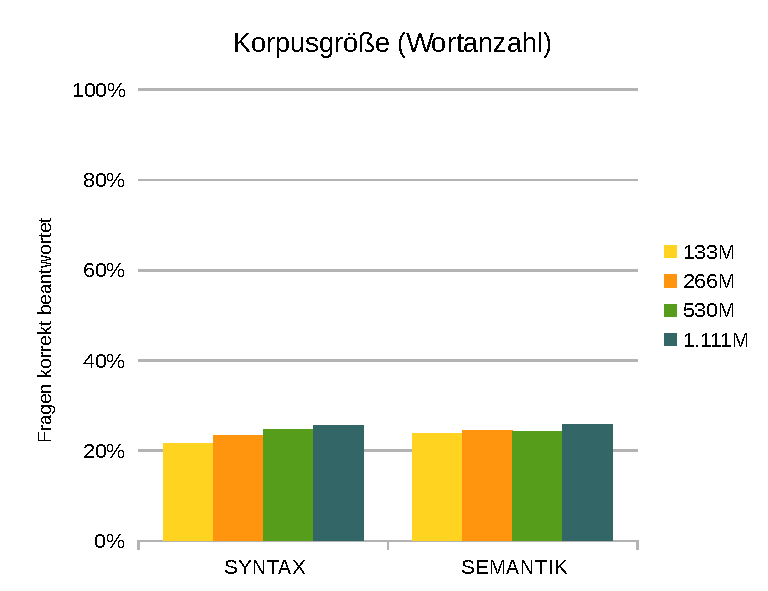
\includegraphics[width=0.52\textwidth]{images/diagram_corpussize_correct}}
% \subcaptionbox{\centering Korrekte Antwort unter den Top 10 Antworten\label{img.diagram_corpussize_top10}}
% {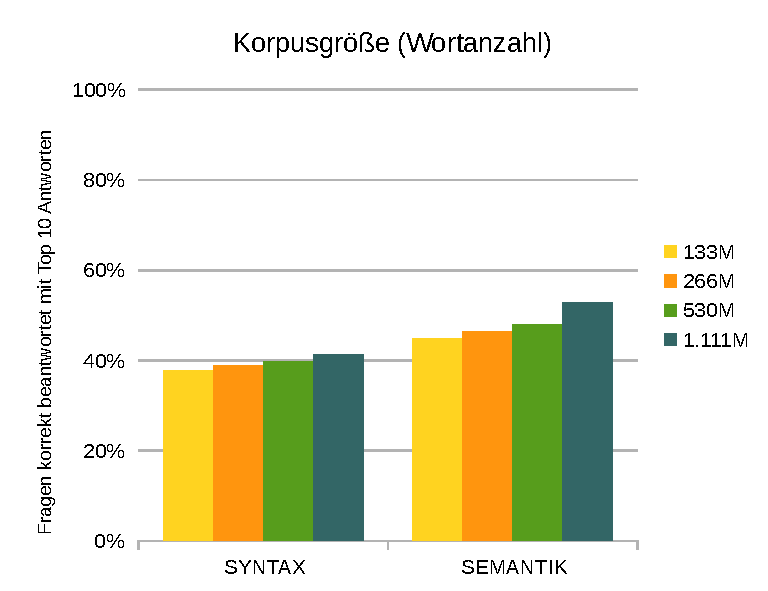
\includegraphics[width=0.52\textwidth]{images/diagram_corpussize_top10}}
% \caption[Gesamtergebnis Korpusgröße]{Gesamtergebnis der Auswirkung der Korpusgröße (Legende vgl. \autoref{tab.preprocessingstats}).}\label{img.diagram_corpussize_all}
% \end{adjustwidth}
% \end{figure}

% \subsection{Korpus Preprocessing}
% Wie in \autoref{s.preprocessing} erläutert, wurden zum Korpus Preprocessing vier Modelle trainiert: Der reine Korpus ohne zusätzliches Preprocessing \code{SG-52-5-RAW}, Filterung von Interpunktion und Stoppwörtern \code{SG-52-5-PS}, zusätzlich dazu die Umwandlung von Umlauten und "s in ihren entsprechenden Digraphen \code{SG-52-5-PSU} und schließlich das Bilden von Bigramm-Tokens \code{SG-52-5-PSUB}. Das Training von \code{SG-52-5-PSUB} ging dabei mit 84 Minuten am schnellsten, bei einer Trainingsgeschwindigkeit von 126k Wörtern pro Sekunde.

% \autoref{img.diagram_preprocessing_correct_all} zeigt das Gesamtergebnis korrekt beantworteter Fragen gruppiert nach Syntaktik und Semantik, \autoref{img.diagram_preprocessing_top10_all} zeigt das Ergebnis für die korrekte Antwort unter den Top 10 Antworten.

% \begin{figure}[H]
% \begin{adjustwidth}{-4mm}{-4mm}
% \centering
% \subcaptionbox{Korrekt beantwortete Fragen\label{img.diagram_preprocessing_correct_all}}
% {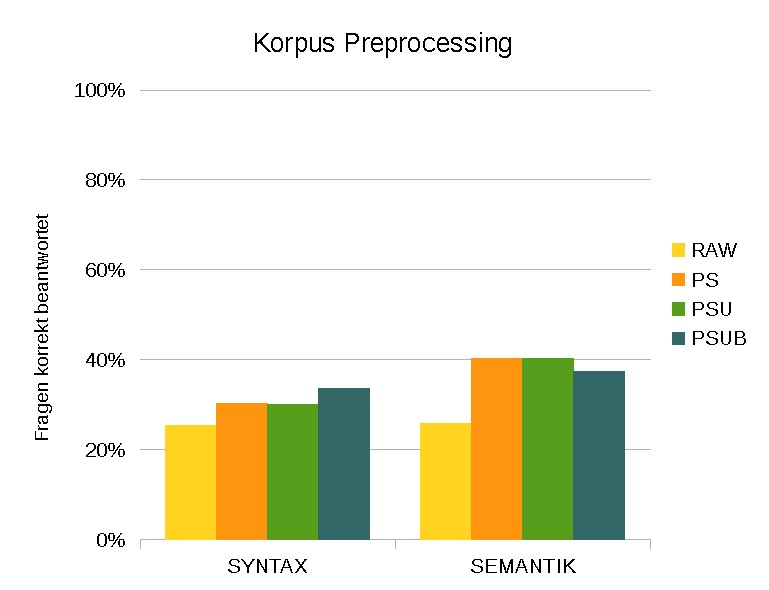
\includegraphics[width=0.52\textwidth]{images/diagram_preprocessing_correct_all}}
% \subcaptionbox{\centering Korrekte Antwort unter den Top 10 Antworten\label{img.diagram_preprocessing_top10_all}}
% {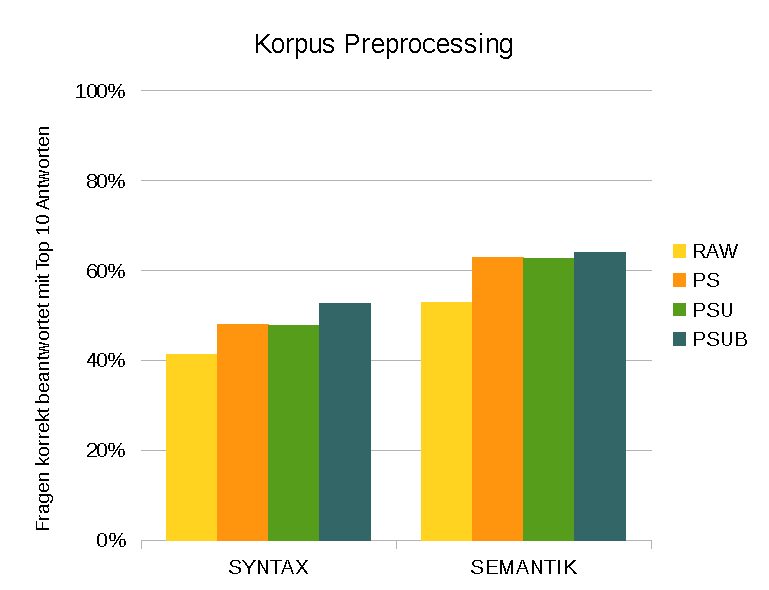
\includegraphics[width=0.52\textwidth]{images/diagram_preprocessing_top10_all}}
% \caption[Gesamtergebnis Korpus Preprocessing]{Gesamtergebnis der Auswirkung des Korpus Preprocessing (Legende vgl. \autoref{tab.preprocessingstats}).}\label{img.diagram_preprocessing_all}
% \end{adjustwidth}
% \end{figure}

% Aus \autoref{img.diagram_preprocessing_correct_all} ist ersichtlich, dass das Modell \code{SG-52-5-PSUB} insgesamt das beste Ergebnis erzielt hat. Hier wurden ein Drittel der Syntaxfragen korrekt beantwortet und bei mehr als der Hälfte dieser Fragen war das korrekte Ergebnis unter den Top 10. Bei den Semantikfragen war die korrekte Antwort sogar bei mehr als 60\% der Fragen unter den Top 10. Anzumerken ist, dass die Modelle \code{SG-52-5-PS} und \code{SG-52-5-PSU} bei der korrekten Antwort von Semantikfragen um etwa 2,5\% besser als \code{SG-52-5 PSUB} abschnitten, dagegen war die Quote der korrekten Antworten unter den Top 10 etwas geringer. Außerdem ergab sich bei beiden Modellen sowohl beim Syntax- als auch beim Semantiktest ein beinahe identisches Ergebnis. Die Umwandlung von Umlauten in ihre Digraph-Repräsentation hatte folglich insgesamt keine Auswirkung auf das Testergebnis.

% \bild{diagram_preprocessing_coverage_all}{0.52\textwidth}{Gesamtdeckung der Test-Set-Fragen der Modelle zum Korpus Preprocessing)}{Evaluation: Gesamtdeckung Korpus Preprocessing}

% Die Deckung der Test-Set-Fragen lag bei allen Modellen bei über 85\%, das Modell ohne zusätzliches Preprocessing wies dabei jeweils eine höhere Deckung auf als die anderen Modelle. Es ist anzunehmen, dass die Ursache hierfür die Filterung der Stoppwörter ist. Beim Semantiktest wurden hier sogar alle Fragen beantwortet. Allgemein war die Deckung des semantischen Test-Sets höher, da dessen Fragen aufgrund der Ausrichtung auf die Wortbedeutung vermutlich weniger Stoppwörter enthalten, als das syntaktische Test-Set.

% \begin{figure}[!ht]
% \begin{adjustwidth}{-4mm}{-4mm}
% \centering
% \subcaptionbox{Korrekt beantwortete Fragen\label{img.diagram_preprocessing_correct_syn}}
% {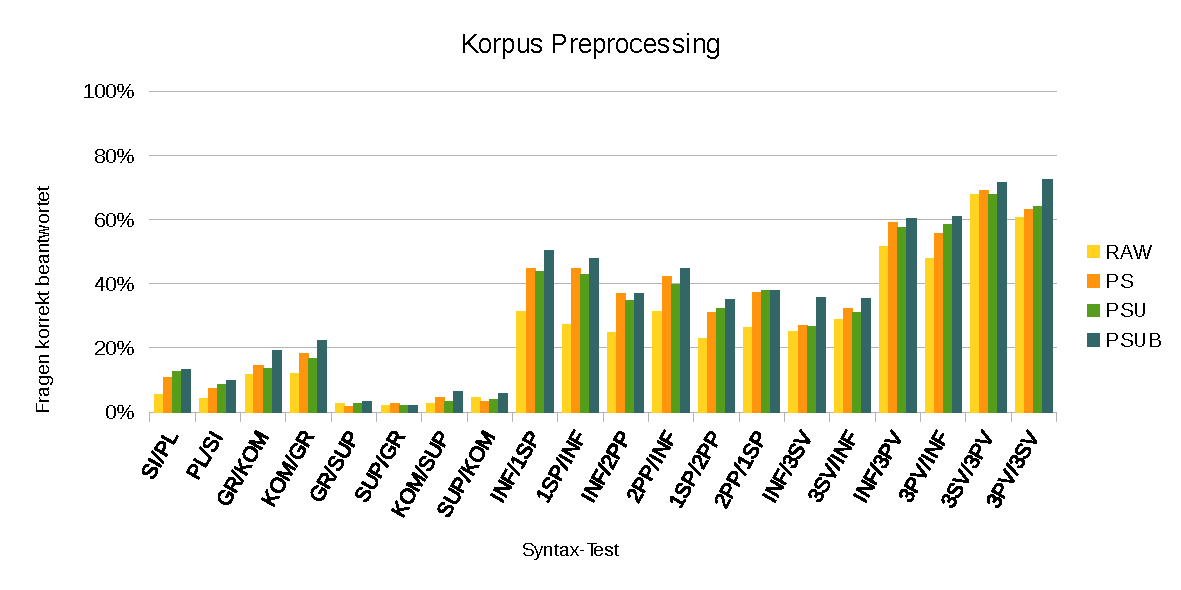
\includegraphics[width=1.04\textwidth]{images/diagram_preprocessing_correct_syn}}
% \subcaptionbox{Korrekte Antwort unter den Top 10 Antworten\label{img.diagram_preprocessing_top10_syn}}
% {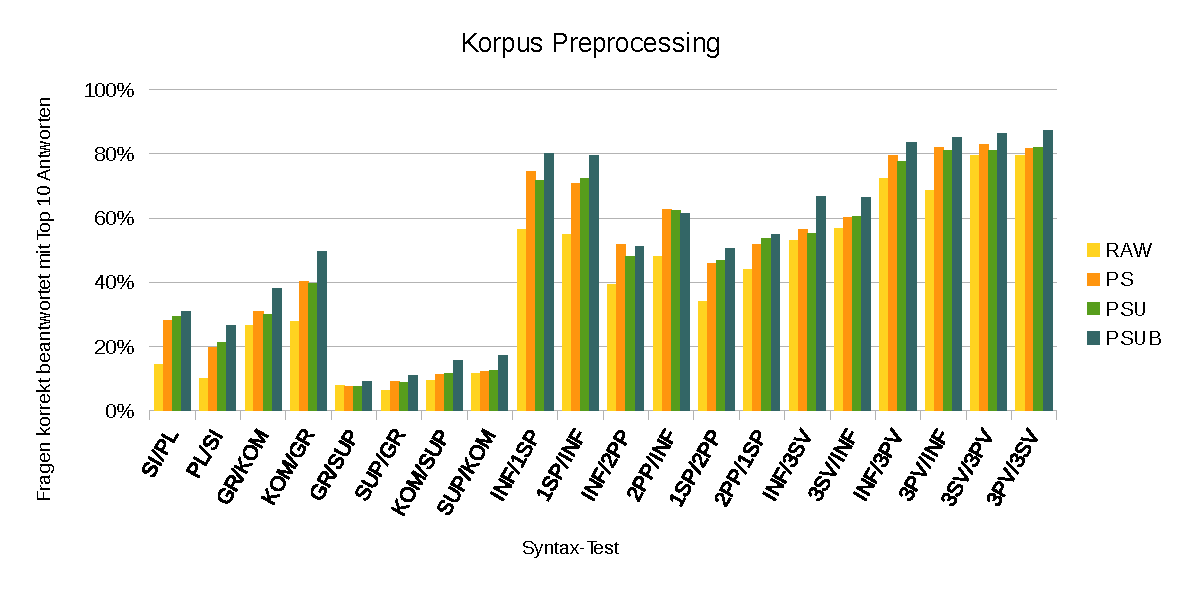
\includegraphics[width=1.04\textwidth]{images/diagram_preprocessing_top10_syn}}
% \caption[Ergebnis der Syntaxfragen Korpus Preprocessing]{Ergebnis der Syntaxfragen Korpus Preprocessing}\label{img.diagram_preprocessing_syn}
% \end{adjustwidth}
% \end{figure}

% Aus der einzelnen Auflistung der syntaktischen Testergebnisse in \autoref{img.diagram_preprocessing_syn} geht zunächst hervor, dass allgemein die Syntax-Fragen zu Nomen und Adjektiven am schlechtesten beantwortet wurden. Insbesondere bei Fragen zum Superlativ von Adjektiven wurden maximal 6\% der Fragen korrekt beantwortet. Betrachtet man die korrekten Antworten unter den Top 10, so wird die Anzahl der korrekt beantworteten Fragen mehr als verdoppelt (vgl. z.B. \tt{SUP/KOM}), teilweise sogar verdreifacht (vgl. z.B. \tt{SUP/GR}). Ursache für dieses Verhalten könnte die Tatsache sein, dass Deutsche Adjektive in ihren Steigerungsformen abhängig von Singular/Plural sind (z.B. \q{der \b{höchste} Turm}, \q{die \b{höchsten} Türme}). Im Englischen gibt es diesen Unterschied nicht (\q{the \b{tallest} tower}, \q{the \b{tallest} towers}). Bei der Evaluierung wird nur eine korrekte Antwort geprüft. Aus diesem Grund fällt das Top 10 Ergebnis deutlich besser aus, da sich die gesuchte Form mit höherer Wahrscheinlichkeit unter den besten 10 Ergebnissen befindet.

% Die besten Ergebnisse der syntaktischen Fragen wurden bei den Verbformen der dritten Person Plural im Präteritum erreicht. In Kombination mit der dritten Person Singular hatten alle Modelle ein Ergebnis von mehr als 60\% und unter den Top 10 mehr als 80\% korrekt beantworteter Fragen.

% \begin{figure}[!ht]
% \centering
% \subcaptionbox{Korrekt beantwortete Fragen\label{img.diagram_preprocessing_correct_sem}}
% {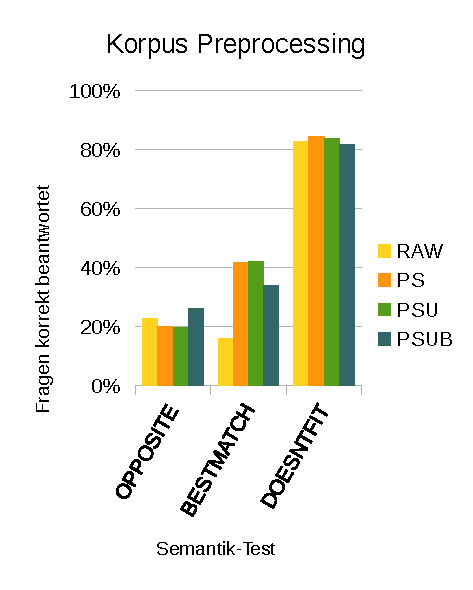
\includegraphics[width=0.4\textwidth]{images/diagram_preprocessing_correct_sem}}
% \subcaptionbox{\centering Korrekte Antwort unter den Top 10 Antworten\label{img.diagram_preprocessing_top10_sem}}
% {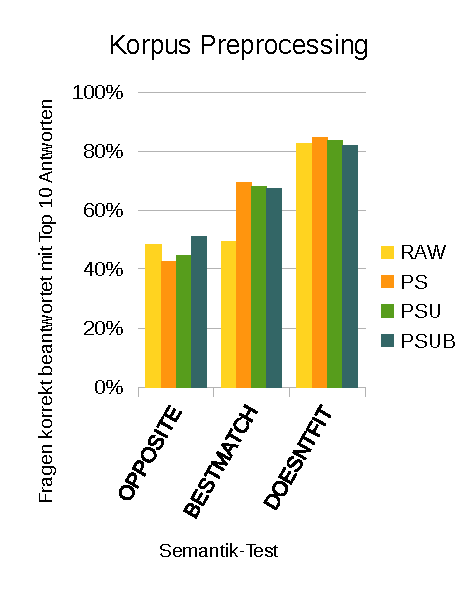
\includegraphics[width=0.4\textwidth]{images/diagram_preprocessing_top10_sem}}
% \caption[Ergebnis der Semantikfragen Korpus Preprocessing]{Ergebnis der Semantikfragen Korpus Preprocessing}\label{img.diagram_preprocessing_sem}
% \end{figure}

% Die Ergebnisse der drei Gruppen der Semantik-Fragen (\autoref{img.diagram_preprocessing_sem}) sind sehr unterschiedlich ausgefallen. Das Gegenteil zu einem gegebenen Wort (\tt{OPPOSITE}) wurde in ca. 20\% der Fälle korrekt gefunden, unter den Top 10 war das richtige Ergebnis bei mehr als 42\% der Fragen. Ähnlich wie bei den Adjektiven ist der Anteil der korrekten Top 10 Antworten damit mehr als doppelt so hoch.
% Beim \tt{BESTMATCH} Test unterscheiden sich die einzelnen Modelle deutlich voneinander. \code{SG-52-5 PS} und \code{SG-52-5 PSU} schneiden dabei mit über 40\% korrekter Antworten mit Abstand am besten ab.
% Beim Test auf das am wenigsten passende Wort in einer Gruppe von 4 Wörtern (\tt{DOESNTFIT}) beantworten schließlich alle 4 Modelle mehr als 4 von 5 Fragen korrekt. Hier sind das Ergebnis korrekter Antworten und das Top 10 Ergebnis identisch, da bei diesem Test kein korrektes Wort aus dem Vokabular gefunden, sondern ein gegebenes Wort identifiziert werden muss.

% \subsection{Skip-Gram Fensterbreite}
% Zur Evaluation verschiedener Fensterbreiten wurden bei konstanter Vektorgröße von 52 vier Modelle mittels Skip-Gram trainiert (\code{SG-52-5}, \code{SG-52-10}, \code{SG-52-15} und \code{SG-52-20}), wobei die Fensterbreite 5, 10, 15 und 20 betrug. Die Trainingsdauer von 84 Minuten bei der Fensterbreite von 5 erhöhte sich dabei mit steigender Fensterbreite nur geringfügig um jeweils etwa 6 Minuten.

% \begin{figure}[H]
% \begin{adjustwidth}{-4mm}{-4mm}
% \centering
% \subcaptionbox{Korrekt beantwortete Fragen\label{img.diagram_sgwindow_correct_all}}
% {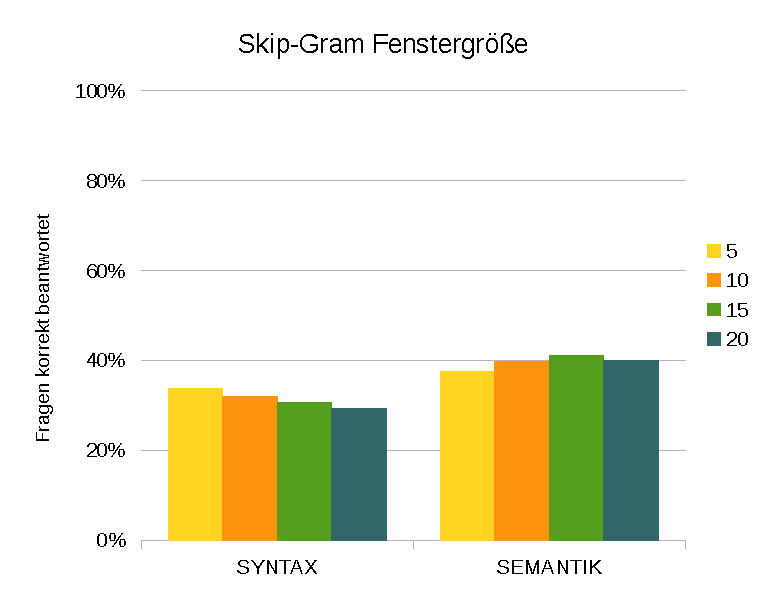
\includegraphics[width=0.52\textwidth]{images/diagram_sgwindow_correct_all}}
% \subcaptionbox{\centering Korrekte Antwort unter den Top 10 Antworten\label{img.diagram_sgwindow_top10_all}}
% {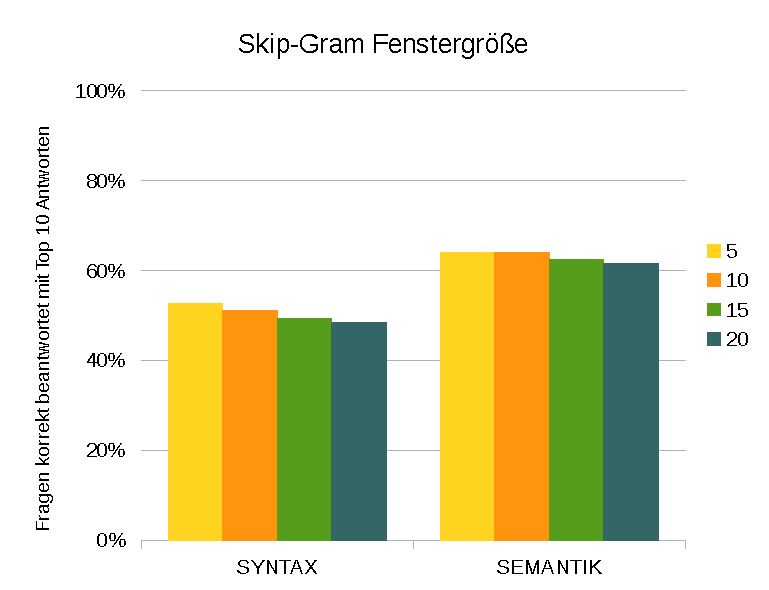
\includegraphics[width=0.52\textwidth]{images/diagram_sgwindow_top10_all}}
% \caption[Gesamtergebnis Skip-Gram Fensterbreite]{Gesamtergebnis Skip-Gram Fensterbreite}\label{img.diagram_sgwindow_all}
% \end{adjustwidth}
% \end{figure}

% Aus \autoref{img.diagram_sgwindow_all} ist ersichtlich, dass das Modell \code{SG-52-5} mit der kleinsten Fensterbreite insgesamt das beste Ergebnis erzielt hat. Im Syntaxtest wurden hier gegenüber den anderen Modellen sowohl die meisten Fragen korrekt beantwortet, als auch die höchste Quote der korrekten Antwort unter den Top 10 Antworten erreicht. Außerdem nimmt die Anzahl korrekter Antworten mit steigender Fensterbreite linear ab. Das gilt auch für die Top 10 Ergebnisse im Semantiktest. Nur beim Test der korrekten Ergebnisse im Semantiktest erzielt das Modell mit Fensterbreite 15 das beste Ergebnis. Folglich könnte eine größere Fensterbreite (zwischen 10 und 20), also das Einbeziehen von Wörtern mit größerem Abstand zum Zielwort, für das korrekte Beantworten semantischer Fragen vorteilhaft sein.

% \subsection{Skip-Gram Vektorgröße}\label{ss.sgvektorgroesse}
% Zur Evaluation verschiedener Vektorgrößen wurden bei konstanter Fensterbreite von 5 und einer Worthäufigkeit von mindestens 10 vier Modelle mittels Skip-Gram trainiert (\code{SG-52-5-R10}, \code{SG-100-5-R10}, \code{SG-200-5-R10} und \code{SG-300-5-R10}), wobei die Vektorgröße 52\footnote{Für die kleinste Vektorgröße wurde 52 statt 50 gewählt, weil die Vektordimension für ein optimales Training ein Vielfaches der verwendeten Threadanzahl (in dieser Arbeit 4) betragen sollte.}, 100, 200 und 300 betrug. Die Trainingsdauer stieg mit steigernder Vektorgröße von 1,4 Stunden (\tt{52}) auf 3,5 Stunden (\tt{300}) stark an.

% \begin{figure}[H]
% \begin{adjustwidth}{-4mm}{-4mm}
% \centering
% \subcaptionbox{Korrekt beantwortete Fragen\label{img.diagram_sgvector_correct_all}}
% {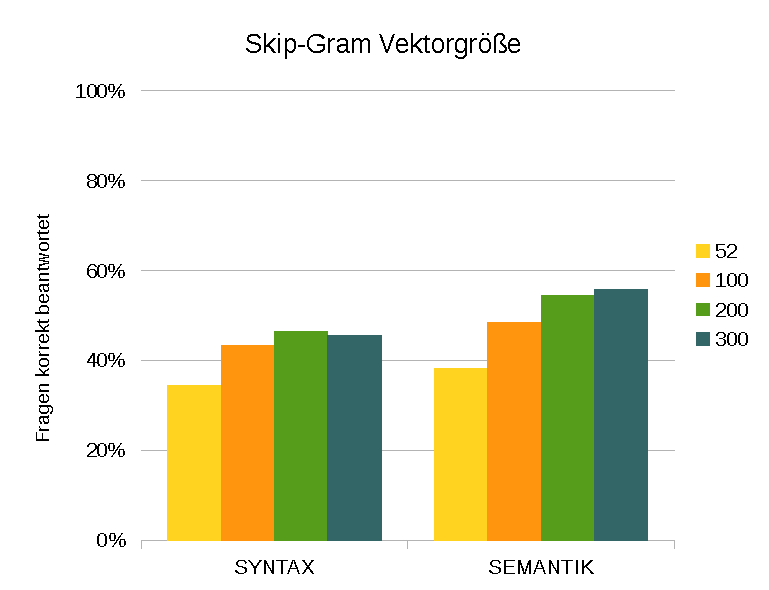
\includegraphics[width=0.52\textwidth]{images/diagram_sgvector_correct_all}}
% \subcaptionbox{\centering Korrekte Antwort unter den Top 10 Antworten\label{img.diagram_sgvector_top10_all}}
% {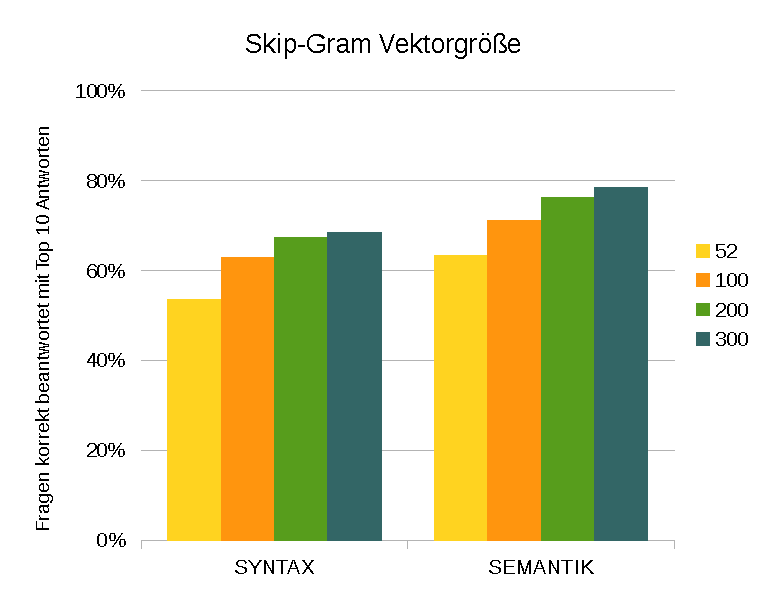
\includegraphics[width=0.52\textwidth]{images/diagram_sgvector_top10_all}}
% \caption[Gesamtergebnis Skip-Gram Vektorgröße]{Gesamtergebnis Skip-Gram Vektorgröße}\label{img.diagram_sgvector_all}
% \end{adjustwidth}
% \end{figure}

% Aus \autoref{img.diagram_sgvector_all} ist ersichtlich, dass das Modell \code{SG-300-5-R10} mit der größten Vektordimension insgesamt das beste Ergebnis erzielt hat. Allgemein nimmt die Anzahl korrekter Antworten mit steigender Vektorgröße zu. Die einzige Ausnahme bildet das Ergebnis der korrekten Antworten beim Syntaxtest (\autoref{img.diagram_sgvector_correct_all} links): Das Modell mit der Vektorgröße 200 ist hier mit einem knappen Vorsprung von 0,9\% das beste Modell.

% \subsection{Continuous-Bag-of-Words Fensterbreite}
% Auch mit der CBOW Architektur wurden vier Modelle unterschiedlicher Fensterbreiten trainiert (\code{CB-52-5}, \code{CB-52-10}, \code{CB-52-15} und \code{CB-52-20}), wobei die Fensterbreite wie bei Skip-Gram 5, 10, 15 und 20 betrug. Die Trainingsdauer war im Gegensatz zu Skip-Gram bei allen Modellen mit ca. 100 Minuten bei einer Trainingsgeschwindigkeit von 105k Wörtern pro Sekunde ungefähr gleich.

% \begin{figure}[!ht]
% \begin{adjustwidth}{-4mm}{-4mm}
% \centering
% \subcaptionbox{Korrekt beantwortete Fragen\label{img.diagram_cbwindow_correct_all}}
% {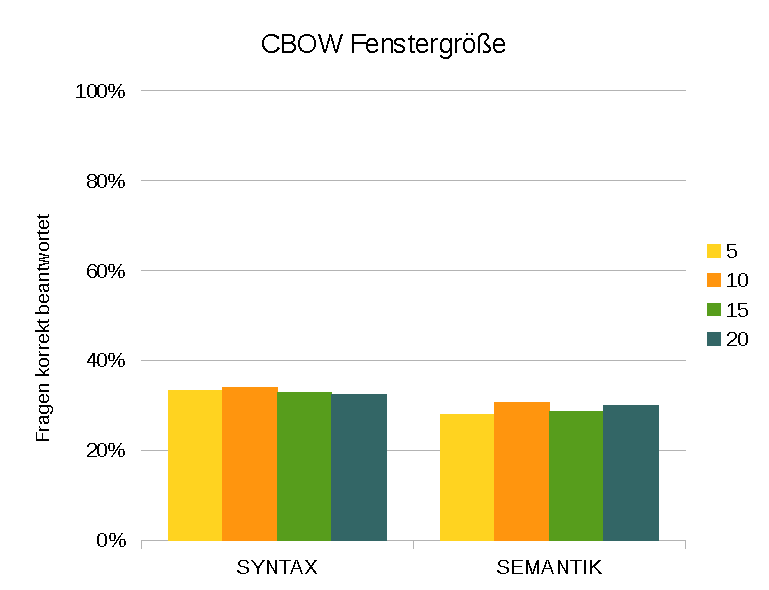
\includegraphics[width=0.52\textwidth]{images/diagram_cbwindow_correct_all}}
% \subcaptionbox{\centering Korrekte Antwort unter den Top 10 Antworten\label{img.diagram_cbwindow_top10_all}}
% {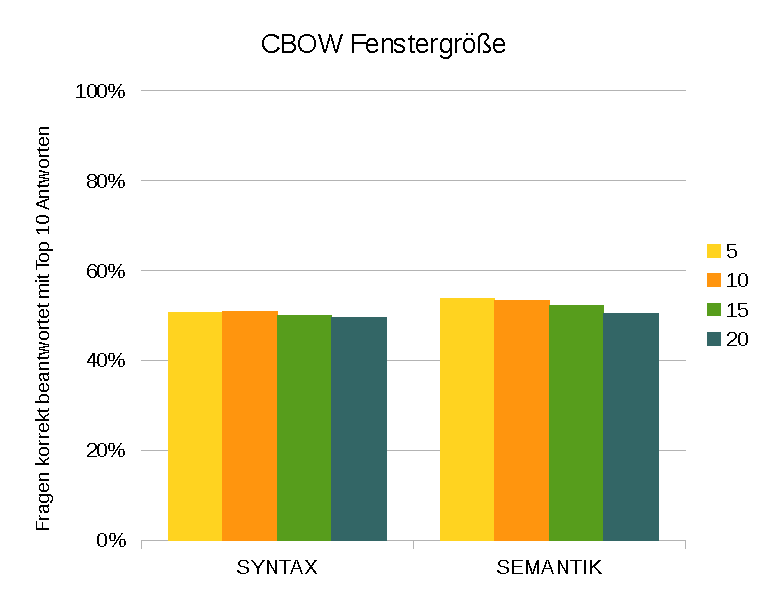
\includegraphics[width=0.52\textwidth]{images/diagram_cbwindow_top10_all}}
% \caption[Gesamtergebnis CBOW Fensterbreite]{Gesamtergebnis CBOW Fensterbreite}\label{img.diagram_cbwindow_all}
% \end{adjustwidth}
% \end{figure}

% Aus \autoref{img.diagram_cbwindow_all} ist ersichtlich, dass bei CBOW im Gegensatz zu Skip-Gram das Modell \code{CB-52-10} mit der Fensterbreite 10 insgesamt das beste Ergebnis erzielt hat.
% Im Syntaxtest wurden hier gegenüber den anderen Modellen sowohl die meisten Fragen korrekt beantwortet, als auch die höchste Quote der korrekten Antwort unter den Top 10 Antworten erreicht. Tendenziell nimmt aber auch hier die Anzahl korrekter Antworten mit steigender Fensterbreite ab.
% Das gilt auch für die Top 10 Ergebnisse im Semantiktest. Nur beim Test der korrekten Ergebnisse unter den Top 10 im Semantiktest erzielt das Modell mit Fensterbreite 5 das beste Ergebnis, allerdings mit einem sehr geringen Vorsprung von 0,3\%.

% \subsection{Skip-Gram Negative Sampling}
% Zur Evaluation der Negative Sampling Optimierung wurden bei konstanter Fensterbreite von 5 und konstanter Vektorgröße von 52 drei Modelle mittels Skip-Gram trainiert (\code{SG-52-5-NS10}, \code{SG-52-5-NS20} und \code{SG-52-5-NS30}), wobei die Anzahl der Negative Samples 10, 20 und 30 betrug. Im Vergleich dazu ist das Modell \code{SG-52-5} ohne Negative Sampling ebenfalls aufgeführt. Die Trainingsdauer der Modelle stieg dabei mit steigender Anzahl der Negative Samples stark an (ca. eine Stunde längeres Training pro zusätzlichen 10 Negative Samples). Das Modell \code{SG-52-5-NS30} benötigte fast 4,5 Stunden für das Training, bei einer Trainingsgeschwindigkeit von 40k Wörtern pro Sekunde.

% \begin{figure}[H]
% \begin{adjustwidth}{-4mm}{-4mm}
% \centering
% \subcaptionbox{Korrekt beantwortete Fragen\label{img.diagram_sgns_correct_all}}
% {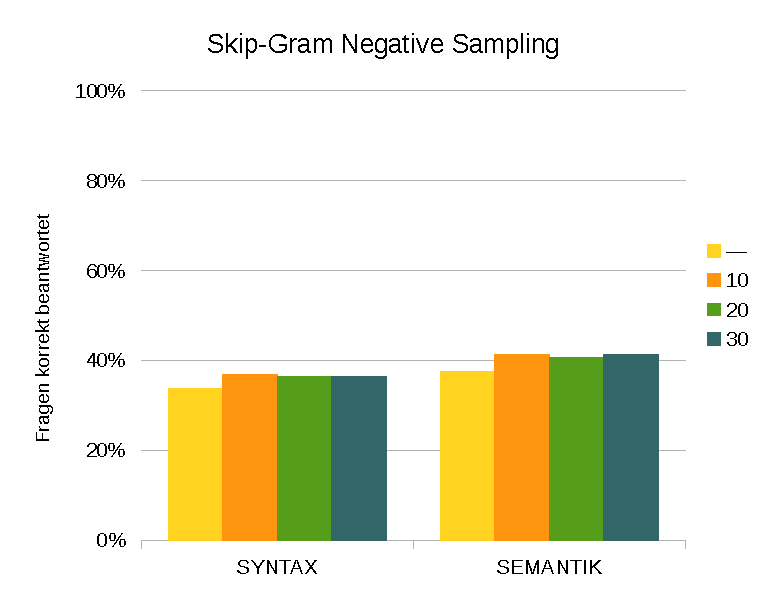
\includegraphics[width=0.52\textwidth]{images/diagram_sgns_correct_all}}
% \subcaptionbox{\centering Korrekte Antwort unter den Top 10 Antworten\label{img.diagram_sgns_top10_all}}
% {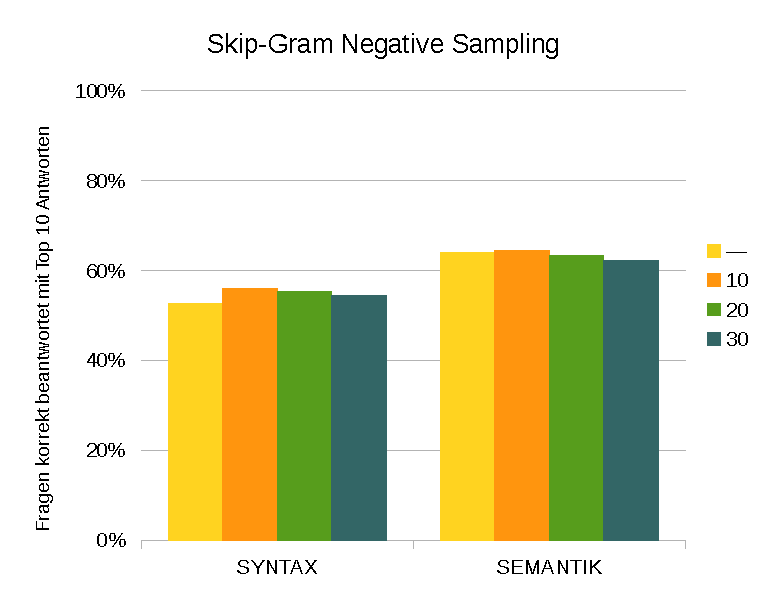
\includegraphics[width=0.52\textwidth]{images/diagram_sgns_top10_all}}
% \caption[Gesamtergebnis Skip-Gram Negative Sampling]{Gesamtergebnis Skip-Gram Negative Sampling. Das erste Modell (---) ist ohne Negative Sampling trainiert.}\label{img.diagram_sgns_all}
% \end{adjustwidth}
% \end{figure}

% Aus \autoref{img.diagram_sgns_all} ist ersichtlich, dass das Modell \code{SG-52-5-NS10} mit der Sample-Anzahl 10 insgesamt das beste Ergebnis erzielt hat. Dabei sind mit Ausnahme der Top 10 Ergebnisse des Semantiktests alle drei Modelle besser als das äquivalente Modell ohne Negative Sampling. Bei der Auswertung der korrekten Antworten in \autoref{img.diagram_sgns_correct_all} sind die Ergebnisse für die unterschiedlichen Sample-Anzahlen annähernd konstant, wohingegen bei der Auswertung der korrekten Antwort unter den Top 10 Antworten in \autoref{img.diagram_sgns_top10_all} ersichtlich ist, dass sich das Ergebnis mit steigender Sample-Anzahl verschlechtert.

% \subsection{Skip-Gram Worthäufigkeit}
% Zur Evaluation der Worthäufigkeit, die ein Wort mindestens erreichen muss, um betrachtet zu werden, wurden bei konstanter Fensterbreite von 5 und konstanter Vektorgröße von 52 vier Modelle mittels Skip-Gram trainiert (\code{SG-52-5-R5}, \code{SG-52-5-R10}, \code{SG-52-5-R20} und \code{SG-52-5-R50}), wobei die Worthäufigkeit mindestens 5, 10, 20 und 50 betrug. Die Trainingsdauer verringerte sich mit steigender Mindestwortanzahl nur geringfügig von 84 Minuten (\tt{R5}) auf 72 Minuten (\tt{R50}), bei einer Trainingsgeschwindigkeit von ungefähr 130k Wörtern pro Sekunde.

% \begin{figure}[H]
% \begin{adjustwidth}{-4mm}{-4mm}
% \centering
% \subcaptionbox{Korrekt beantwortete Fragen\label{img.diagram_sgrw_correct_all}}
% {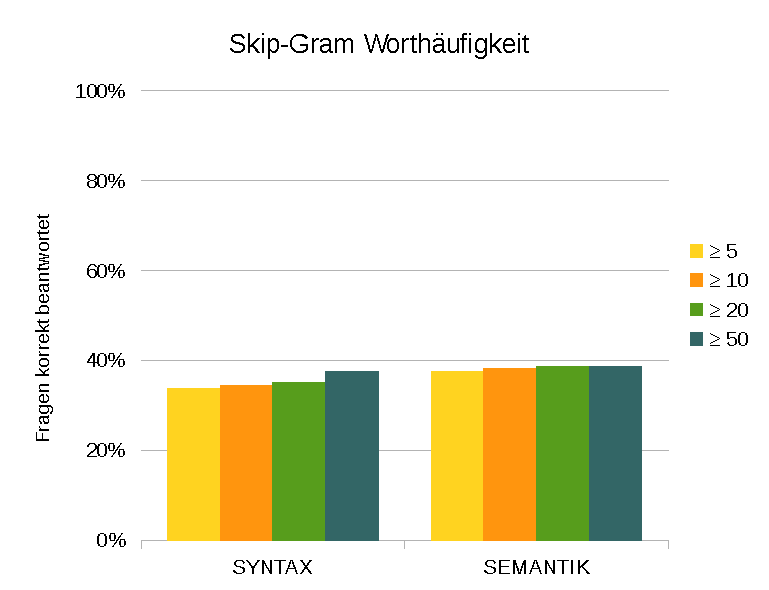
\includegraphics[width=0.52\textwidth]{images/diagram_sgrw_correct_all}}
% \subcaptionbox{\centering Korrekte Antwort unter den Top 10 Antworten\label{img.diagram_sgrw_top10_all}}
% {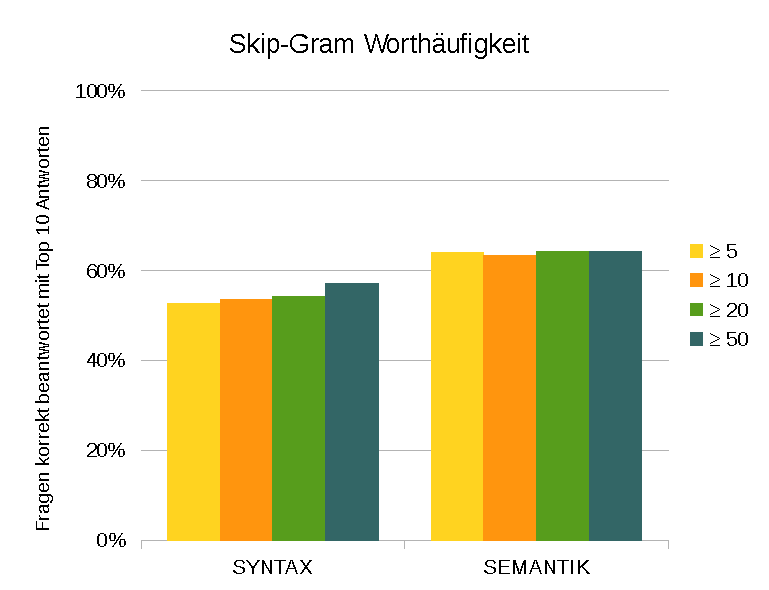
\includegraphics[width=0.52\textwidth]{images/diagram_sgrw_top10_all}}
% \caption[Gesamtergebnis Skip-Gram Worthäufigkeit]{Gesamtergebnis Skip-Gram Worthäufigkeit}\label{img.diagram_sgrw_all}
% \end{adjustwidth}
% \end{figure}

% Aus \autoref{img.diagram_sgrw_all} ist ersichtlich, dass das Modell \code{SG-52-5-R50} mit einer Worthäufigkeit von mindestens 50 insgesamt das beste Ergebnis erzielt hat. Dabei sind die Ergebnisse des Semantiktests für alle Modelle beinahe identisch, wohingegen beim Syntaxtest eindeutig das Modell mit einer Worthäufigkeit von mindestens 50 das beste Ergebnis erzielt.

% \bild{diagram_sgrw_coverage_all}{0.52\textwidth}{Gesamtdeckung der Test-Set-Fragen der Modelle zur Worthäufigkeit}{Evaluation: Gesamtdeckung Worthäufigkeit}

% Aufgrund des Aussortierens von Wörtern niedrigerer Häufigkeit, verringert sich die Deckung der Test-Set-Fragen (dargestellt in \autoref{img.diagram_sgrw_all}) mit steigender Mindest-Worthäufigkeit geringfügig. Dies wirkt sich allerdings nur auf die Deckung der Syntaxfragen aus. Anzunehmen ist, dass diese Verringerung der Deckung die Anzahl falscher Antworten vermindert und somit für die Verbesserung des qualitativen Ergebnisses des Syntaxtestes verantwortlich ist.

% \subsection{Architektur, Projektion und Hierarchical Softmax}
% In der letzten Evaluationsgruppe wurden die Architekturen CBOW und Skip-Gram miteinander verglichen. Dabei wurde bei den CBOW-Modellen die Projektionsart variiert (Summe oder Durchschnitt) und die Skip-Gram-Modelle wurden einmal mit und einmal ohne Hierarchical Sampling trainiert. Das Evaluationsergebnis ist in \autoref{img.diagram_cbsmsg_all} abgebildet.

% \begin{figure}[!ht]
% \begin{adjustwidth}{-4mm}{-4mm}
% \centering
% \subcaptionbox{Korrekt beantwortete Fragen\label{img.diagram_cbsmsg_correct_all}}
% {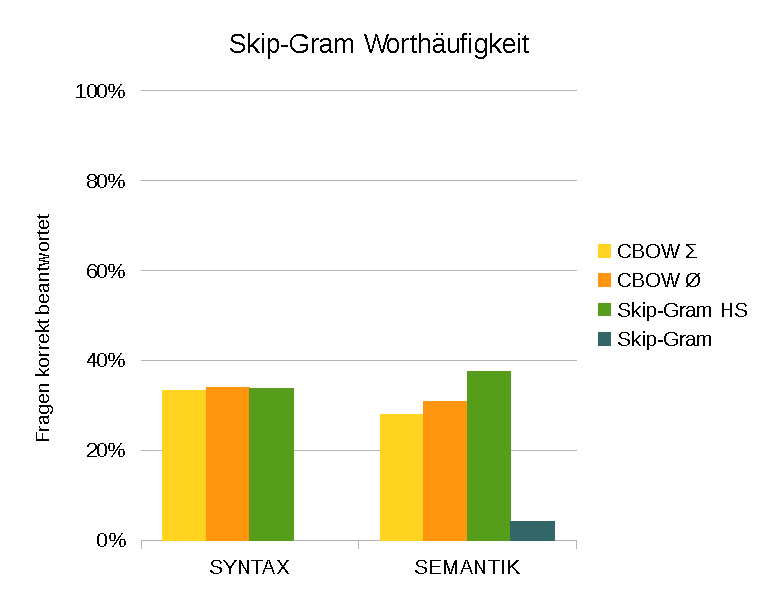
\includegraphics[width=0.52\textwidth]{images/diagram_cbsmsg_correct_all}}
% \subcaptionbox{\centering Korrekte Antwort unter den Top 10 Antworten\label{img.diagram_cbsmsg_top10_all}}
% {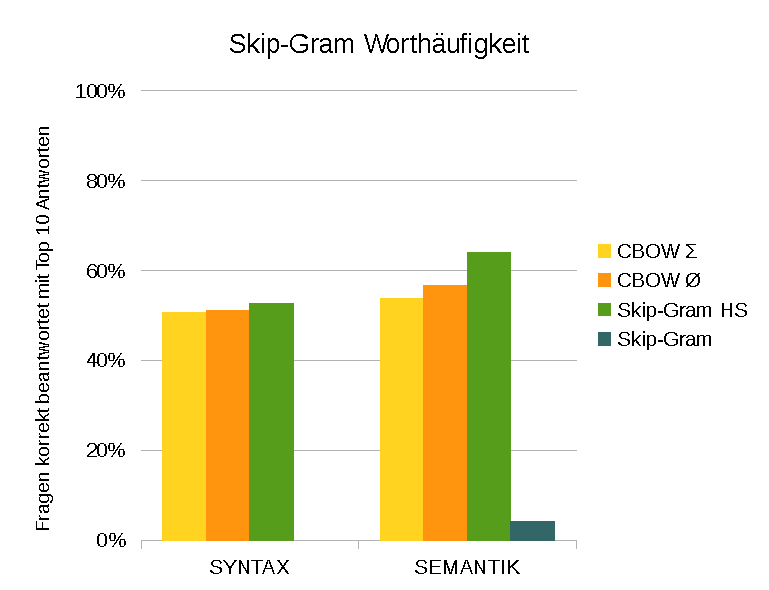
\includegraphics[width=0.52\textwidth]{images/diagram_cbsmsg_top10_all}}
% \caption[Gesamtergebnis Architektur, Projektion und Hierarchical Softmax]{Gesamtergebnis Architektur, Projektion und Hierarchical Softmax}\label{img.diagram_cbsmsg_all}
% \end{adjustwidth}
% \end{figure}

% Zunächst fällt auf, dass das Skip-Gram-Modell ohne Hierarchical Softmax keine einzige Syntaxfrage und nur 4,2\% der Semantikfragen korrekt beantworten konnte. Bei den beiden CBOW-Modellen erzielt das Modell mit der Projektion der Wort-Vektoren durch Bilden des Durchschnitts sowohl im Syntax- als auch im Semantiktest das bessere Ergebnis. Im Gesamtergebnis liefert jedoch das Skip-Gram-Modell mit Hierarchical Softmax das beste Ergebnis, im Semantiktest sogar mit einem Abstand von über 7\%.

% \section{Diskussion optimaler Parameter}\label{s.parameterspezifikation}
% Basierend auf den Evaluationsergebnissen der einzelnen Evaluationsgruppen, welche in \autoref{s.testergebnis} erläutert wurden, kann nun die Parameterkonfiguration für das im Rahmen dieser Arbeit optimale Deutsche Sprachmodell spezifiziert werden. Dazu ist die aus der Parameterkonfiguration bekannte \autoref{tab.parameter} als Übersicht mit dem jeweils besten Modell einer Gruppe (markiert) in \autoref{tab.bestparameter} dargestellt.

% \begin{table}[!ht]\vspace{1ex}\small\centering\def\arraystretch{1.0}\begin{tabular}{|l|l|l|c|c|c|c|c|c|}
% \hline Modellname & A         & Pr         & D   & N  & HS   & NS   & R  & P \\ \hline\hline
% \tt{SG-52-5-133M} & Skip-Gram & ---        & 52  & 5  & Ja   & Nein & 5  & ---    \\ \hline
% \tt{SG-52-5-266M} & Skip-Gram & ---        & 52  & 5  & Ja   & Nein & 5  & ---    \\ \hline
% \tt{SG-52-5-530M} & Skip-Gram & ---        & 52  & 5  & Ja   & Nein & 5  & ---    \\ \hline\rowcolor{lightgreen}
% \tt{SG-52-5-1B}   & Skip-Gram & ---        & 52  & 5  & Ja   & Nein & 5  & ---    \\ \hline\hline
% \tt{SG-52-5-RAW}  & Skip-Gram & ---        & 52  & 5  & Ja   & Nein & 5  & ---    \\ \hline
% \tt{SG-52-5-PS}   & Skip-Gram & P, S       & 52  & 5  & Ja   & Nein & 5  & ---    \\ \hline
% \tt{SG-52-5-PSU}  & Skip-Gram & P, S, U    & 52  & 5  & Ja   & Nein & 5  & ---    \\ \hline\rowcolor{lightgreen}
% \tt{SG-52-5-PSUB} & Skip-Gram & P, S, U, B & 52  & 5  & Ja   & Nein & 5  & ---    \\ \hline\hline\rowcolor{lightgreen}
% \tt{SG-52-5}      & Skip-Gram & P, S, U, B & 52  & 5  & Ja   & Nein & 5  & ---    \\ \hline
% \tt{SG-52-10}     & Skip-Gram & P, S, U, B & 52  & 10 & Ja   & Nein & 5  & ---    \\ \hline
% \tt{SG-52-15}     & Skip-Gram & P, S, U, B & 52  & 15 & Ja   & Nein & 5  & ---    \\ \hline
% \tt{SG-52-20}     & Skip-Gram & P, S, U, B & 52  & 20 & Ja   & Nein & 5  & ---    \\ \hline\hline
% \tt{SG-52-5-R10}  & Skip-Gram & P, S, U, B & 52  & 5  & Ja   & Nein & 5  & ---    \\ \hline
% \tt{SG-100-5-R10} & Skip-Gram & P, S, U, B & 100 & 5  & Ja   & Nein & 5  & ---    \\ \hline
% \tt{SG-200-5-R10} & Skip-Gram & P, S, U, B & 200 & 5  & Ja   & Nein & 5  & ---    \\ \hline\rowcolor{lightgreen}
% \tt{SG-300-5-R10} & Skip-Gram & P, S, U, B & 300 & 5  & Ja   & Nein & 5  & ---    \\ \hline\hline
% \tt{CB-52-5}      & CBOW      & P, S, U, B & 52  & 5  & Ja   & Nein & 5  & $\sum$ \\ \hline\rowcolor{lightgreen}
% \tt{CB-52-10}     & CBOW      & P, S, U, B & 52  & 10 & Ja   & Nein & 5  & $\sum$ \\ \hline
% \tt{CB-52-15}     & CBOW      & P, S, U, B & 52  & 15 & Ja   & Nein & 5  & $\sum$ \\ \hline
% \tt{CB-52-20}     & CBOW      & P, S, U, B & 52  & 20 & Ja   & Nein & 5  & $\sum$ \\ \hline\hline
% \tt{SG-52-5}      & Skip-Gram & P, S, U, B & 52  & 5  & Ja   & Nein & 5  & ---    \\ \hline\rowcolor{lightgreen}
% \tt{SG-52-5-NS10} & Skip-Gram & P, S, U, B & 52  & 5  & Ja   & 10   & 5  & ---    \\ \hline
% \tt{SG-52-5-NS20} & Skip-Gram & P, S, U, B & 52  & 5  & Ja   & 20   & 5  & ---    \\ \hline
% \tt{SG-52-5-NS30} & Skip-Gram & P, S, U, B & 52  & 5  & Ja   & 30   & 5  & ---    \\ \hline\hline
% \tt{SG-52-5}      & Skip-Gram & P, S, U, B & 52  & 5  & Ja   & Nein & 5  & ---    \\ \hline
% \tt{SG-52-5-R10}  & Skip-Gram & P, S, U, B & 52  & 5  & Ja   & Nein & 10 & ---    \\ \hline
% \tt{SG-52-5-R20}  & Skip-Gram & P, S, U, B & 52  & 5  & Ja   & Nein & 20 & ---    \\ \hline\rowcolor{lightgreen}
% \tt{SG-52-5-R50}  & Skip-Gram & P, S, U, B & 52  & 5  & Ja   & Nein & 50 & ---    \\ \hline\hline
% \tt{CB-52-5-SUM}  & CBOW      & P, S, U, B & 52  & 5  & Ja   & Nein & 5  & $\sum$ \\ \hline
% \tt{CB-52-5-MEAN} & CBOW      & P, S, U, B & 52  & 5  & Ja   & Nein & 5  & \O     \\ \hline\rowcolor{lightgreen}
% \tt{SG-52-5-HS}   & Skip-Gram & P, S, U, B & 52  & 5  & Ja   & Nein & 5  & ---    \\ \hline
% \tt{SG-52-5-NOHS} & Skip-Gram & P, S, U, B & 52  & 5  & Nein & Nein & 5  & ---    \\ \hline
% \end{tabular}
% \caption[Parameter-Spezifikationen trainierter Modelle nach Evaluation]{\label{tab.bestparameter}Parameter-Spezifikationen trainierter Modelle zur Architektur $A$, Preprocessing $Pr$, Vektordimension $D$, Fensterbreite $N$, Hierarchical Softmax $HS$, Negative Sampling $NS$, Worthäufigkeit $R$ und Projektionsart $P$. Markierte Modelle lieferten das beste Evaluationsergebnis ihrer Gruppe.}
% \vspace{1ex}\end{table}

% Daraus sind folgende Spezifikationen ersichtlich:

% Der Trainingskorpus sollte möglichst groß sein und vorverarbeitet werden, indem Interpunktion und Stoppwörter gefiltert und Bigramm-Tokens gebildet werden; als Trainingsarchitektur sollte Skip-Gram gewählt werden; die Fensterbreite sollte zwischen 5 und 10 liegen; die Vektordimension sollte je nach verfügbarer Rechenleistung möglichst groß gewählt werden; Negative Sampling sollte bei einer vergleichsweise kleinen Sample-Anzahl von 10 verwendet werden; Wörter mit geringer Häufigkeit ($\leq$ 50) sollten für qualitativ bessere Ergebnisse gefiltert werden\footnote{Dabei ist allerdings darauf zu achten, dass die Deckung der Test-Set-Fragen noch ausreichend hoch ist.}; Hierarchical Sampling sollte verwendet werden.

% \section{Auswertung des optimalen Modells}\label{s.optimalesmodell}
% Im Folgenden werden die Ergebnisse des Modells mit der in \autoref{s.parameterspezifikation} gefundenen optimalen Parameterkonfiguration vorgestellt und mit den Ergebnissen von Mikolov et al. \citep{Mikolov2012} für ein englisches Modell verglichen. Das Training dieses Modells dauerte dabei ungefähr 6 Stunden bei einer Trainingsgeschwindigkeit von knapp 27k Wörtern pro Sekunde.

% \subsection{Evaluationsergebnis}\label{ss.evaluationsergebnis}

% Das Gesamtergebnis des optimalen Modells in \autoref{img.diagram_optimal_all} zeigt den Anteil korrekt beantworteter Fragen mit der ersten Antwort und mit den Top 10 Antworten. Im Syntaxtest wurden über die Hälfte der Fragen korrekt beantwortet, im Semantiktest sogar 60\%. Die korrekte Antwort lag unter den Top 10 Antworten bei 3 von 4 Fragen im Syntaxtest und bei 4 von 5 Fragen im Semantiktest. Das ist im Hinblick auf das eigenständige Lernen sprachlicher Strukturen (unüberwachtes Training) ein sehr gutes Ergebnis.

% \bild{diagram_optimal_all}{0.6\textwidth}{Gesamtergebnis des optimalen Modells}{Evaluation: Gesamtergebnis optimales Modell}

% In \autoref{tab.comparison} ist der Vergleich der Evaluationsergebnisse des Syntaxtests mit dem englischen Modell \tt{RNN-1600} von Mikolov et al. dargestellt. Dieses Modell wurde mithilfe eines Recurrent-Netzwerks auf englischen Nachrichtenartikeln mit insgesamt 320 Millionen Wörtern trainiert, bei einer Vektordimension von 1600.

% \begin{table}[!ht]\vspace{1ex}\small\centering\def\arraystretch{1.1}\begin{tabular}{|l|c|c|c|c|}
% \hline Sprach-Modell & Adjektive & Nomen & Verben & Gesamt \\ \hline\hline
% Deutsch (diese Arbeit) & \b{27,4} &    23,3  & \b{68,6} & \b{52,3} \\ \hline
% Englisch (RNN-1600)    &    23,9  & \b{29,2} &    62,2  &    39,6  \\ \hline
% \end{tabular}
% \caption[Vergleich: deutsches und englisches Sprachmodell]{\label{tab.comparison}Vergleich der Ergebnisse des Syntaxtests des besten deutschen Modells dieser Arbeit mit dem besten englischen Modell von Mikolov et al. \citep{Mikolov2012}. Angaben in Prozent.}
% \vspace{1ex}\end{table}

% Anzumerken ist hier, dass der direkte Vergleich der Evaluationsergebnisse beider Modelle aus unterschiedlichen Gründen nicht vollständig repräsentativ ist. Zum einen wurden unterschiedliche Korpora für das Training verwendet. Dies ist für den sprachlichen Unterschied zwar notwendig, trotzdem können dabei Größe und Bezugsquelle des Korpus übereinstimmen. In dieser Arbeit wurden sowohl deutsche Nachrichtenartikel als auch die deutsche Wikipedia mit insgesamt über 650 Millionen Wörtern als Korpus verwendet, Mikolov et al. nutzen dagegen ausschließlich Nachrichtenartikel bei weniger als der Hälfte der Wörter (320 Millionen). Zum anderen wurden verschiedene Test-Sets für die Evaluation genutzt, wobei sowohl die Gesamtanzahl der Fragen, als auch die Anzahl der Fragen zu den unterschiedlichen Wortarten (Adjektive, Nomen und Verben) verschieden war \footnote{Für den Syntaxtest wurden im englischen Modell 8k Fragen verwendet, jeweils 3k für Adjektive und Verben und 2k für Nomen \citep{Mikolov2012}.}.

% Trotz der beschriebenen Einschränkungen des Modellvergleichs ist ersichtlich, dass sprachliche Zusammenhänge ähnlich abgebildet werden. So beantworten beide Modelle die Fragen zu Adjektiven und Nomen zu höchstens 30\% korrekt, wobei die Antworten der Fragen zu Verben über 60\% korrekt waren. Dies lässt die Schlussfolgerung zu, dass sowohl in englischen als auch in deutschen Modellen Verben besser abgebildet werden als Nomen und Adjektive.

% \subsection{Ausgewählte Wortzusammenhänge}\label{ss.wortzusammenhaenge}
% Nachdem die Modelle allgemein ausgewertet wordem somd, beschäftigt sich dieser Abschnitt mit ausgewählten konkreten Beispielen komplexerer Wortzusammenhänge, die mithilfe zusätzlicher Analogiefragen manuell gefunden werden konnten. Damit wird die Fähigkeit der Wort-Vektoren verdeutlicht, die Bedeutung von Wörtern abbilden zu können. Wie bereits bei den Analogiefragen der Evaluation wurde eine Vektoraddition (bzw. -subtraktion) vollzogen und anschließend der Vektor ausgegeben, der dem Ergebnis am ähnlichsten ist. Eine Auswahl davon wird im Folgenden beschrieben. Die Kosinusähnlichkeit (vgl. \autoref{ss.bagofwords}) ist jeweils in Klammern angegeben.

% \code{Frau + Kind = Mutter} (0,831)\\
% Ein sehr häufig auftretender familiärer Zusammenhang mit einer vergleichsweise hohen Kosinusähnlichkeit.

% \code{Verwaltungsgebaeude + Buecher = Bibliothek} (0,718)\\
% Der Zusammenhang von Gebäudearten und ihrer Funktion, in diesem Fall ein Gebäude zur Verwaltung von Büchern.

% \code{Haus + Filme + Popcorn = Kino} (0,721)\\
% Eine weiteres Beispiel einer Gebäudeart. Interessant ist hier, dass bereits der Vektor \tt{Haus + Filme} dem Vektor \tt{Kino} am ähnlichsten ist, hier allerdings mit einer etwas geringeren Kosinusähnlichkeit von 0,713. Das bedeutet, dass das Hinzufügen von \tt{Popcorn} den Vektor \tt{Kino} besser beschreibt.

% \code{Planet + Wasser = Erde} (0,717)\\
% Das Hauptmerkmal unseres Planeten gegenüber anderer Planeten wird korrekt erkannt.

% \code{Kerze + Feuerzeug = brennende\_Kerze} (0,768)\\
% Schließlich ein Beispiel für ein Bigramm. Ohne die Umformung der Korpusdaten zu Bigrammen könnte diese Beziehung so nicht dargestellt werden.

% \subsection{Visualisierung mit Principal Component Analysis}\label{ss.pca}
% Neben der Darstellung von Wortbedeutungen mithilfe der Analogiefragen ist es auch möglich, Merkmale von Wort-Vektoren zu visualisieren, um gelernte sprachliche Konzepte zu verdeutlichen.

% Die Anzahl der Dimensionen der Wort-Vektoren sollte für eine bessere Modellierung von Sprache möglichst groß gewählt werden (vgl. Evaluationsergebnisse der Vektorgröße in \autoref{ss.sgvektorgroesse}). Dabei ist es jedoch unmöglich, einen solch hochdimensionalen Vektor direkt grafisch darzustellen. Aus diesem Grund gibt es die \i{Principal Component Analysis} (PCA, deutsch: Hauptkomponentenanalyse, begründet von Karl Pearson, 1901 \citep{Pearson1901}). PCA ist eine statistische Analysemethode, welche die hohe Komponentenanzahl einer Variablen auf einige wenige Hauptkomponenten reduzieren kann, welche die ursprüngliche Variable möglichst aussagekräftig beschreiben. Mikolov et al. \citep{Mikolov2013Dist} haben die Beziehung zwischen Land und Hauptstadt mittels PCA für ein englisches Sprachmodell dargestellt.

% \begin{figure}[!ht]
% \begin{adjustwidth}{-4mm}{-4mm}
% \centering
% \subcaptionbox{\centering Abbildung von Ländern und ihren Hauptstädten\label{img.pca_capital}}
% {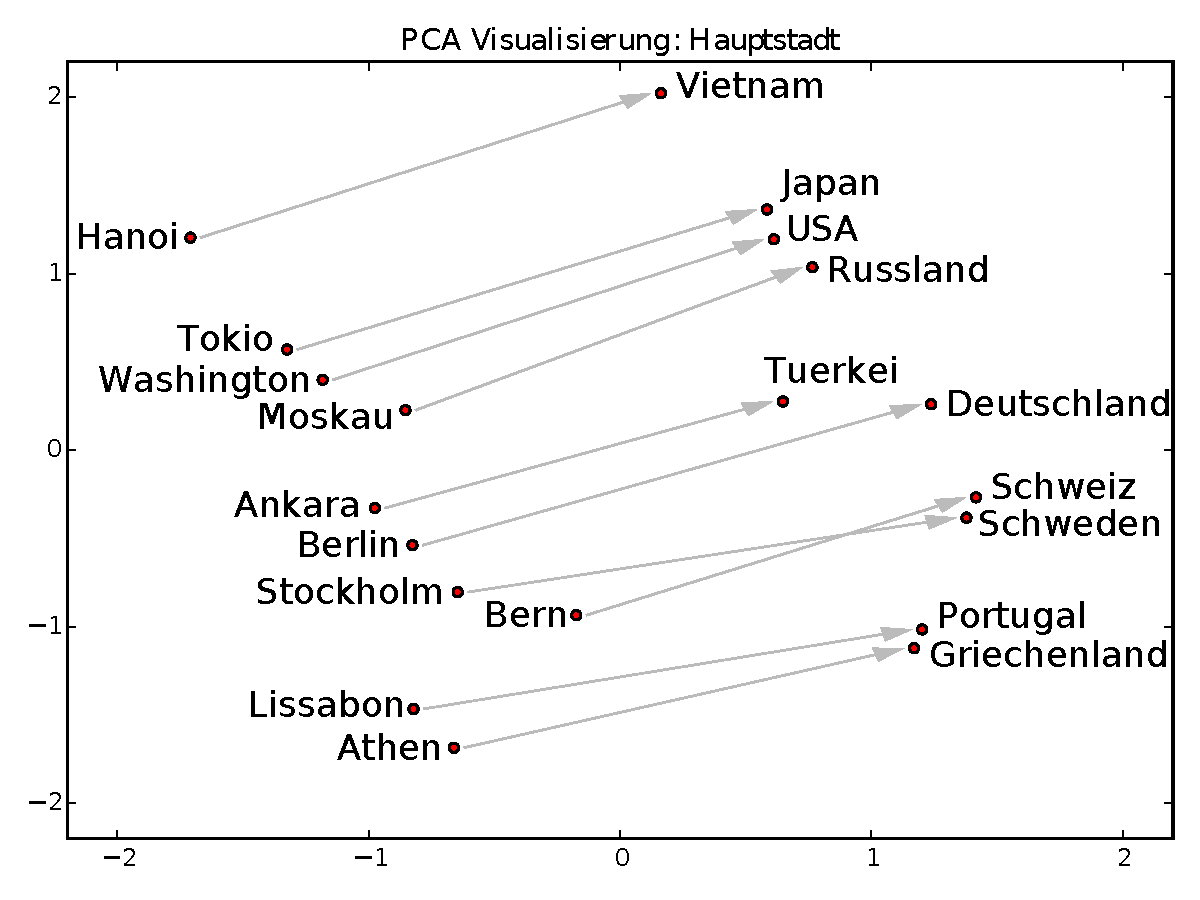
\includegraphics[width=0.52\textwidth]{images/pca_capital}}
% \subcaptionbox{\centering Abbildung von Ländern und ihren Währungen\label{img.pca_currency}}
% {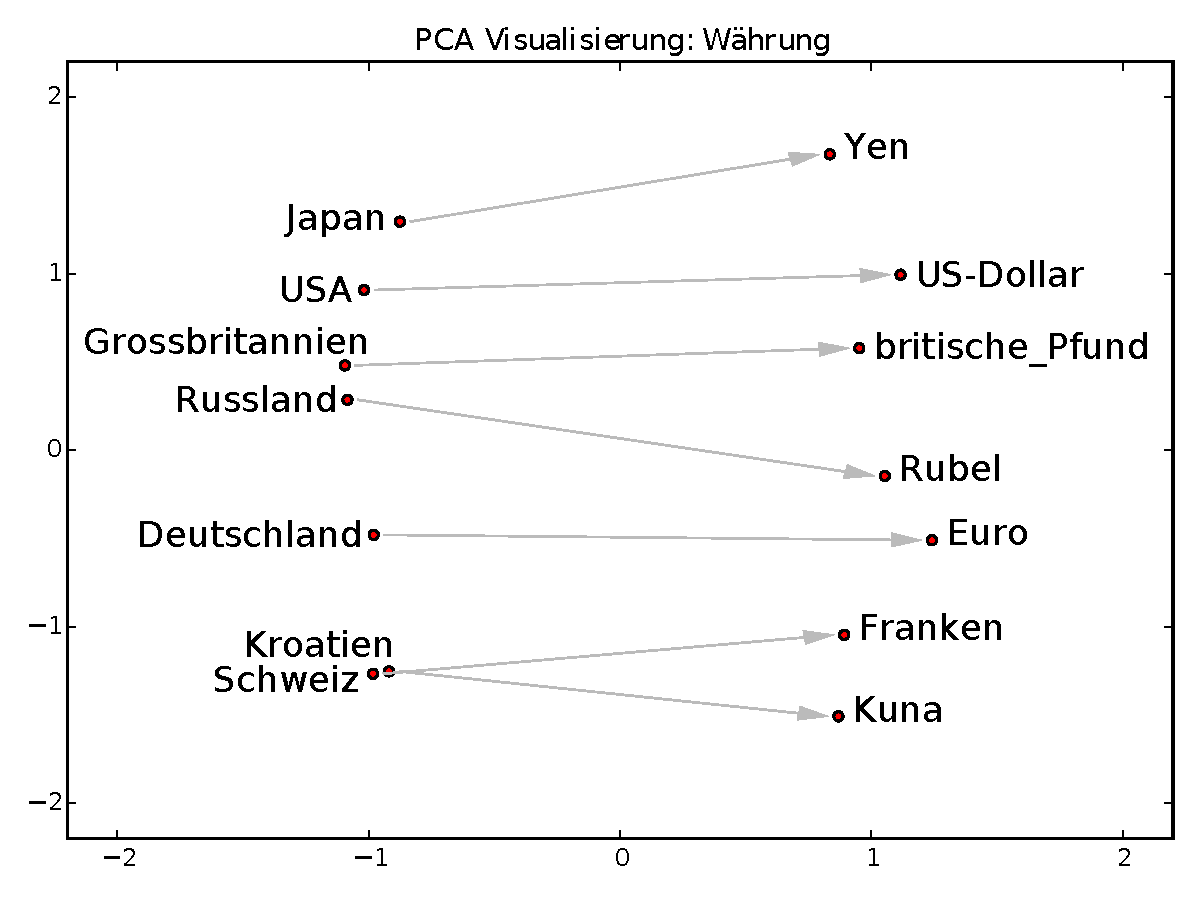
\includegraphics[width=0.52\textwidth]{images/pca_currency}}
% \subcaptionbox{\centering Abbildung von Ländern und ihren Sprachen\label{img.pca_language}}
% {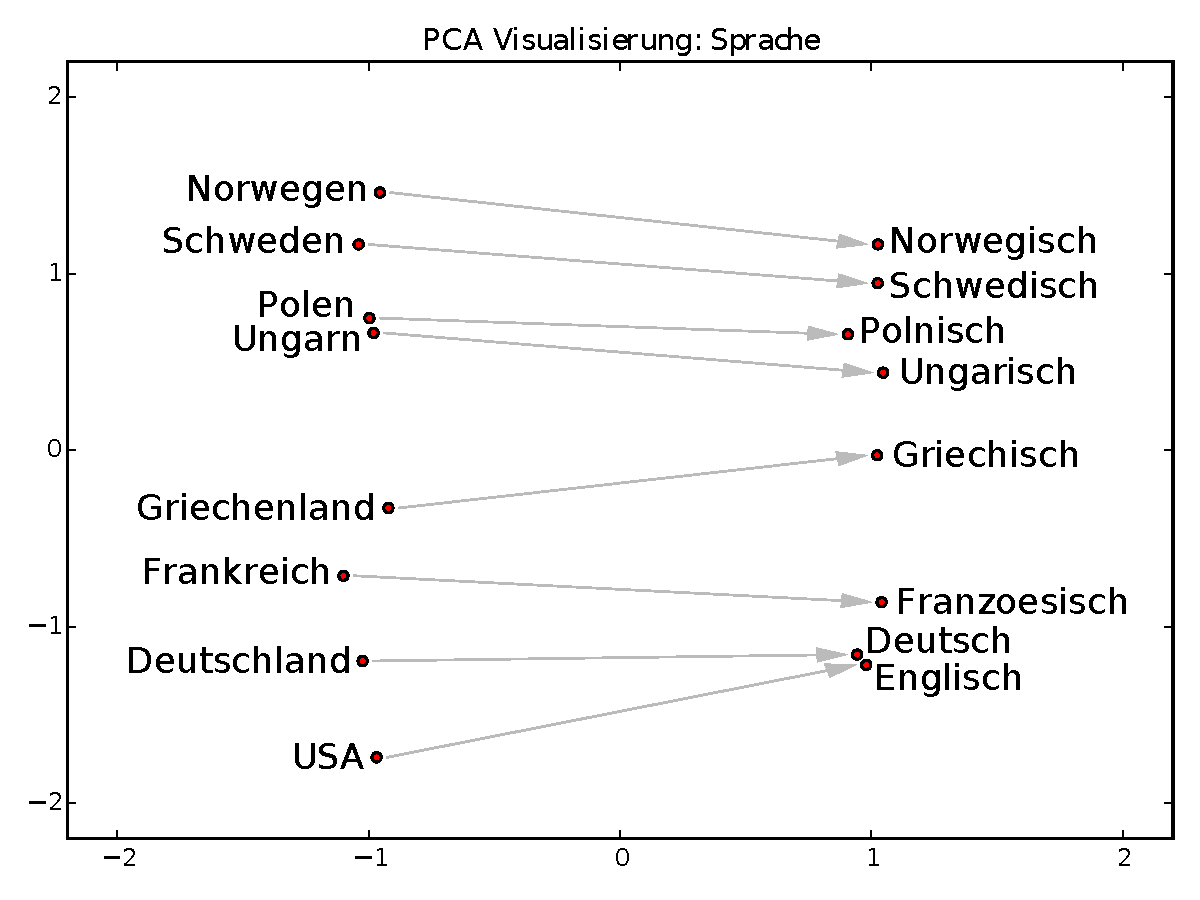
\includegraphics[width=0.52\textwidth]{images/pca_language}}
% \caption[PCA Visualisierung von Wort-Vektoren]{PCA Visualisierung von Wort-Vektoren von Ländern, Hauptstädten, Währungen und Sprachen}\label{img.pca}
% \end{adjustwidth}
% \end{figure}

% Die Größe der Wort-Vektoren des optimalen Modells in dieser Arbeit ist 300. Diese Größe wurde mithilfe von PCA auf 2 Dimensionen reduziert und für ausgewählte Wort-Vektoren in \autoref{img.pca} dargestellt. Dabei wurden manuell Länder mit ihren entsprechenden Hauptstädten, Währungen und Sprachen ausgewählt. Aufgrund der zweidimensionalen Darstellung ist sehr gut ersichtlich, dass das Sprachmodell z.B. in \autoref{img.pca_language} das Konzept von Landessprachen gelernt hat, ohne dass im Training explizit vorgegeben wurde, welches die Sprache eines Landes ist (unüberwachtes Training). In der Abbildung sind Länder links und entsprechende Sprachen rechts gruppiert zu sehen. Der Abstand und die Verbindungsrichtung eines Landes zu seiner Sprache sind dabei untereinander sehr ähnlich. Genauso ist diese Gruppierung auch für Hauptstädte und Währungen zu beobachten.

% \subsection{Verteilung korrekter Antworten}\label{ss.verteilungkorrekterantworten}
% Ein weiterer interessanter Aspekt der Evaluation des optimalen Modells ist die Anzahl korrekter Antworten in Abhängigkeit von den ersten $N$ als korrekt geltenden Antworten (Top N).

% In \autoref{img.diagram_topn} ist der Anteil korrekt beantworteter Syntaxfragen in Abhängigkeit der Anzahl $N$ der als korrekt geltenden Antworten abgebildet. Dabei ist ersichtlich, dass für kleine $N$ ($\leq 10$) der Anteil korrekt beantworteter Fragen mit steigendem $N$ stark zunimmt. Für größere $N$ flacht der Anstieg immer mehr ab, sodass sich das Ergebnis schließlich durch Erhöhung von $N$ nicht mehr verbessert. Das bedeutet, dass sich eine mögliche korrekte Antwort mit hoher Wahrscheinlichkeit auch unter den ersten Ergebnissen befindet, welche das Modell liefert.

% \bild{diagram_topn}{0.7\textwidth}{Anteil korrekt beantworteter Syntaxfragen des optimalen Modells unter Variation der Anzahl $N$ der als korrekt geltenden Antworten (Top N)}{Evaluation: Top N}

% In diesem Kapitel wurden die Ergebnisse dieser Arbeit präsentiert und verschiedene Modelle mittels selbst generierter Test-Sets auf allgemeiner Ebene evaluiert. Außerdem wurde das daraus resultierende optimale Modell im Vergleich zu ähnlichen Experimenten und anhand konkreter Beispiele ausgewertet. Im Folgenden wird abschließend zu diesen Ergebnissen Stellung genommen.

% ==================================================================================================
\chapter{Fazit}\label{c.fazit}
Zur Verarbeitung großer Textmengen und automatisierter Modellierung von Sprache gibt es viele Ansätze. Dabei erreicht \i{Deep Learning} mithilfe neuronaler Netzwerke basierend auf englischer Sprache heute nicht nur hervorragende Ergebnisse, sondern kann Modelle mithilfe von Architekturen wie Skip-Gram oder CBOW auch unüberwacht trainieren.

Während das Trainieren von Wort-Vektoren bisher hauptsächlich für die englische Sprache durchgeführt wurde, hat diese Arbeit gezeigt, dass eine solche Sprachmodellierung auch für die deutsche Sprache funktioniert. Es wurden mithilfe eines dafür entwickelten Toolkits unter Parametervariation insgesamt 25 unterschiedliche Modelle und daraus resultierend ein optimales Modell trainiert\footnote{Dieses deutsche Sprachmodell, das entwickelte Toolkit und die generierten Test-Set Fragen stehen für weiterführende Anwendungen zum freien Download zur Verfügung. Müller, Andreas (o.J.), URL: \url{http://devmount.github.io/GermanWordEmbeddings} (Stand: 30.06.2015)}, welches bei der Evaluierung syntaktischer Merkmale ein ähnliches Niveau erreicht, wie ein vergleichbares System (vgl. \autoref{ss.evaluationsergebnis}). Dieses Training war dabei aufgrund einer recheneffizienten Implementierung von Skip-Gram und CBOW auch auf großen Korpora mit einem normalen Heimrechner (vgl. \autoref{ss.trainingsumgebung}) möglich. Beliebige und große Korpora konnten verwendet werden, da das Training unüberwacht stattfand und deshalb keine gelabelten Eingabedaten nötig waren, sondern ausschließlich Text, wie er im normalen Sprachgebrauch auftritt.

Mit der aus der Analyse der Evaluationsergebnisse gefundenen optimalen Parameterkofiguration konnten die im Rahmen dieser Arbeit besten deutschen Wort-Vektoren trainiert werden. Mit diesen Wort-Vektoren war es möglich, syntaktische und semantische Wort-Zusammenhänge darzustellen, komplexe Wortbeziehungen in ihrer Bedeutung korrekt zuordnen (vgl. \autoref{ss.wortzusammenhaenge}) und Merkmale mithilfe von PCA zu visualisieren.

Die in dieser Arbeit trainierten Wort-Vektoren können nun als Grundlage für weiterführende Forschungen und Anwendungen der Sprachmodellierung für die deutsche Sprache dienen, wie z.B. \i{Relation Detection} bzw. \i{Relation Classification} (das Modellieren und anschließende Klassifizieren der Beziehung von Wörtern zueinander) oder \i{Sentiment Analysis} (das Erkennen positiver oder negativer Aussagen).

% ==================================================================================================
% Anhang
\appendix
\chapter{Anhang}

\section{Training}
\begin{multicols}{8}
[\captionof{lstlisting}{Liste der im Training verwendeten Deutschen Stoppwörter des Natural Language Toolkit (NLTK)}]%
\lstinputlisting[language=C, numbers=none, xleftmargin=0em, label={lst.stopwords}]{data/german.stopwords}
\end{multicols}

\section{Test-Sets}
\begin{multicols}{2}
[\captionof{lstlisting}{Syntaktische Analogiefragen (Auszug): Eine Frage (bestehend aus zwei Wortpaaren) pro Zeile, Zeile beginnend mit Doppelpunkt ist das Label des Test-Musters.}]%
\lstinputlisting[language=C, numbers=none, xleftmargin=0em, label={lst.testset_syn}]{data/syntactic.questions.excerpt}
\end{multicols}
\begin{multicols}{2}
[\captionof{lstlisting}{Thematische Analogiefragen (Auszug): Eine Frage (bestehend aus zwei Wortpaaren) pro Zeile.}]%
\lstinputlisting[language=C, numbers=none, xleftmargin=0em, label={lst.testset_sembm}]{data/semantic_bm.questions.excerpt}
\end{multicols}
\begin{multicols}{2}
[\captionof{lstlisting}{Fragen zum inhaltlich nicht passenden Wort einer Wortreihe (Auszug): Eine Frage (bestehend aus drei zueinander passenden Wörtern und einem nicht passenden vierten Wort) pro Zeile.}]%
\lstinputlisting[language=C, numbers=none, xleftmargin=0em, label={lst.testset_semdf}]{data/semantic_df.questions.excerpt}
\end{multicols}
\begin{multicols}{3}
[\captionof{lstlisting}{Analogiefragen zum Gegenteil eines Wortes (Auszug): Eine Frage (bestehend aus zwei Wortpaaren) pro Zeile.}]%
\lstinputlisting[language=C, numbers=none, xleftmargin=0em, label={lst.testset_semop}]{data/semantic_op.questions.excerpt}
\end{multicols}

% \begin{multicols}{2}
% [\captionof{lstlisting}{Generieren von Test-Sets - \tt{evaluation.py}}]%
% \lstinputlisting[language=Python, label={lst.evaluation}]{../GermanWordEmbeddings/evaluation.py}
% \end{multicols}

% \bibliographystyle{apalike}
% \bibliographystyle{plainnat}
% \bibliographystyle{abbrvnat}
% \bibliographystyle{unsrtnat}
% \bibliographystyle{alphadin}
\bibliographystyle{plain}
\bibliography{bibliographie}

\end{document}